%%%% Modèle proposé par kira.ribeiro@universite-paris-saclay.fr  %%%%
%%%% màj : 27/01/2023 %%%%

\documentclass{maThese}

\usepackage{lipsum} % à retirer!!!
\begin{document}

\begin{titlepage}

%\thispagestyle{empty}

\newgeometry{left=6cm,bottom=2cm, top=1cm, right=1cm}

\tikz[remember picture,overlay] \node[opacity=1,inner sep=0pt] at (-13mm,-135mm){\includegraphics{Frame-ups.pdf}};

%*****************************************************
%******** NUMÉRO D'ORDRE DE LA THÈSE À COMPLÉTER *****
%******** POUR LE SECOND DÉPOT                   *****
%*****************************************************

\color{white}

\begin{picture}(0,0)
\put(-152,-743){\rotatebox{90}{\Large \textsc{THESE DE DOCTORAT}}} \\
\put(-120,-743){\rotatebox{90}{NNT : 2020UPASA001}}
\end{picture}
 
%*****************************************************
%******************** TITRE **************************
%*****************************************************

\flushright
\vspace{10mm} % à régler éventuellement
\color{Prune}

\fontsize{22}{26}\selectfont
  \Huge Méthodes d’analyse comparée des pangénomes procaryotes : \\ explorer la diversité génomique inter-espèces pour une meilleure  compréhension du métabolisme \\

\normalsize
\color{black}
\Large{\textit{Methods for comparative analysis of prokaryotic pangenomes: exploring interspecies genomic diversity for a better understanding of metabolism}} \\
%*****************************************************


\fontsize{8}{12}\selectfont

\vspace{1.5cm}

\normalsize
\textbf{Thèse de doctorat de l'université Paris-Saclay} \\

\vspace{6mm}

\small École doctorale n$^{\circ}$ 577, STRUCTURE ET DYNAMIQUE DES SYSTÈMES VIVANTS (SDSV)\\
\small Spécialité de doctorat : Sciences de la vie et de la santé\\
\small Graduate School : Life Sciences and Health. Référent : Université d’Évry Val d’Essonne \\
\vspace{6mm}

\footnotesize Thèse préparée dans la (ou les) unité(s) de recherche \textbf{Université Paris-Saclay, Univ Evry, CNRS, CEA, Génomique métabolique, 91057, Evry-Courcouronnes, France.}, sous la direction de \textbf{David Vallenet}, Directeur de recherche CEA, Genoscope CEA, la co-direction de \textbf{Alexandra Calteau}, Chercheure CEA, Genoscope CEA\\
\vspace{15mm}

\textbf{Thèse soutenue à Paris-Saclay, le 19 mai 2025, par}\\
\bigskip
\Large {\color{Prune} \textbf{Jérôme ARNOUX}} % Changer le Prénom et le NOM

%************************************
\vspace{\fill} % ALIGNER LE TABLEAU EN BAS DE PAGE
%************************************

\bigskip

\flushleft
\small {\color{Prune} \textbf{Composition du jury}}\\
{\color{Prune} \scriptsize {Membres du jury avec voix délibérative}} \\
\vspace{2mm}
\scriptsize
\begin{tabular}{|p{7cm}l}
\arrayrulecolor{Prune}
\textbf{Lucie BITTNER} &  Rapportrice \\ 
Maîtresse de conférence, Sorbonne Université   &   \\ 
\textbf{François Sabot} &  Rapporteur \\ 
Directeur de recherche, université de Montpellier  &   \\ 
\textbf{Stéphanie BURY-MONÉ} & Examinatrice\\ 
Professeure, Université Paris Saclay & \\
\textbf{Jean CURY} &  Examinateur \\ 
Chercheur, Institut Pasteur   &   \\
\end{tabular} 
\vspace{2mm}

\begin{tabular}{p{7cm}l}
\textbf{Alexandra CALTEAU} & Invitée\\ 
Chercheuse, CEA & \\
\textbf{David Vallenet} & Invité\\ 
Directeur de recherche, CEA & \\
\end{tabular} 

\end{titlepage}



% page des résumés à garder en 2ème page. Si les résumés sont trop longs pour tenir sur une seule et même page, on peut mettre un résumé par page
\thispagestyle{empty}
\newgeometry{top=1.5cm, bottom=1.25cm, left=2cm, right=2cm}


\noindent 
%*****************************************************
%***** LOGO DE L'ED À CHANGER IMPÉRATIVEMENT *********
%*****************************************************
\includegraphics[height=2.45cm]{images/logos/logo_usp_SDSV.png}
\vspace{1cm}
%*****************************************************

\small

\begin{mdframed}[linecolor=Prune,linewidth=1]

\textbf{Titre:} Méthodes d’analyse comparée des pangénomes procaryotes : explorer la diversité génomique inter-espèces pour une meilleure  compréhension du métabolisme

\noindent \textbf{Mots clés:} 3 à 6 mots clefs (version en français)

\vspace{-.5cm}
\begin{multicols}{2}
\noindent \textbf{Résumé:}\lipsum[1-2] 
\end{multicols}

\end{mdframed}

\vspace{8mm}

\begin{mdframed}[linecolor=Prune,linewidth=1]

\textbf{Title:} Methods for comparative analysis of prokaryotic pangenomes: exploring interspecies genomic diversity for a better understanding of metabolism

\noindent \textbf{Keywords:} 3 à 6 mots clefs (version en anglais)

\begin{multicols}{2}
\noindent \textbf{Abstract:} \lipsum[1-2]
\end{multicols}
\end{mdframed}

\newgeometry{top=4cm, bottom=4cm, left=2cm, right=2cm}

\tableofcontents

\newgeometry{top=4cm, bottom=4cm, left=4cm, right=4cm}

\newgeometry{top=4cm, bottom=4cm, left=2cm, right=2cm}

\listoffigures

\newgeometry{top=4cm, bottom=4cm, left=4cm, right=4cm}

\newgeometry{top=4cm, bottom=4cm, left=2cm, right=2cm}

\listoftables

\newgeometry{top=4cm, bottom=4cm, left=4cm, right=4cm}

% \newgeometry{top=4cm, bottom=4cm, left=2cm, right=2cm}
% \addcontentsline{toc}{chapter}{Acronymes}
% \printacronyms[title = \centering Acronymes]

% \newgeometry{top=4cm, bottom=4cm, left=4cm, right=4cm}

% \newgeometry{top=4cm, bottom=4cm, left=2cm, right=2cm}

% \addcontentsline{toc}{chapter}{Glossaire}
% \printglossary

% \newgeometry{top=4cm, bottom=4cm, left=4cm, right=4cm}

\chapter*{Introduction}
\addcontentsline{toc}{chapter}{Introduction}

Cette introduction a pour objectifs de faire le panorama scientifique et historique des différents sujets qui seront abordés dans ce manuscrit de thèse. Elle fait aussi place d'entrée en matière pour les personnes non expertes qui liront ce manuscrit. Pour ces quelques lignes, je me permettrais donc quelques facilités et imprécisions scientifiques, que j'espère me seront pardonnées.
\newline

L'origine de la vie sur Terre est encore pleine de question et de débat scientifique passionnant. Néanmoins, les premières traces de vie remontent à 4 milliards d'années et correspondent à des microorganismes, des êtres invisibles à l'{\oe}il nu. Ces microorganismes colonisent la Terre depuis des milliards d'années et représentent aujourd'hui la proportion d'être vivant la plus importante en termes de nombre et de diversité. Ils jouent un rôle crucial dans les écosystèmes, les cycles biogéochimiques et la santé de la planète comme de la nôtre. Pourtant, la microbiologie, l'étude des microorganismes, reste une science relativement récente. Même s'il existe bien, dans l'Antiquité, certains savants et philosophes qui avaient déjà imaginé ces "animaux invisibles", marquant une compréhension primitive de la transmission des maladies infectieuses, il faudra attendre l'invention du microscope par Leeuwenhoek, au XVIIe siècle, pour qu'il fasse les premières observations d'\textit{animaculum}, marquant la naissance de la microbiologie. La microbiologie du XVIIe au XXe siècle à amener de grandes découvertes et révolution scientifique, notamment en médecine. Nous pouvons citer les travaux de Louis Pasteur qui a prouvé que les maladies infectieuses étaient causées par des microorganismes, ou encore d'Alexander Fleming qui découvrit la pénicilline, le premier antibiotique. 


En s'éloignant quelque peu de la microbiologie, toujours entre le XVIIe et XXe siècle, les chimistes s'intéressent aux molécules du vivant. Le Français Antoine Fourcroy va faire la première description de substances azotées dans les organismes vivants, qu'il appelait "substances animales". Ce sont ensuite les chimistes suédois et néerlandais Jöns Jacob Berzelius et Gérardus Johannes Mulder, qui ont introduit le terme "protéine". Le mot vient du grec \textit{proteios}, qui signifie "de première importance", soulignant l'importance fondamentale de ces molécules composées de carbone, hydrogène, azote et oxygène, avec des proportions spécifiques, dans les organismes vivants. Enfin, en 1894, le chimiste allemand, Emil Fischer, démontra que les protéines sont composées d'acides aminés, unité de base des protéines, liés par des liaisons peptidiques. Il déterminera la composition et la structure de plusieurs d'entre eux. La fin du XIXe siècle voit aussi la découverte d'un autre molécule du vivant, l'acide désoxyribonucléique, mieux connue sous l'acronyme ADN. C'est le biologiste suisse Friedrich Miescher qui découvre une substance riche en phosphore dans les cellules du pus, qu'il appelle "nucléine". Il faudra attendre près d'un demi-siècle pour que Phoebus Levene, biochimiste russe-américain, identifie les composants de base de l'ADN : les nucléotides. Plus tard, en pleine Seconde Guerre mondiale, les chercheurs Oswald Avery, Colin MacLeod et Maclyn McCarty, confirment l'hypothèse de Miescher, en montrent que l’ADN est la substance qui transfère les caractères héréditaires et que l'ADN est le support de l’information génétique. Pour terminer, les travaux de Watson et Crick, sans oublier la contribution de Rosalind Franklin, a permis de décrire la structure de la molécule d'ADN. Toutes ces découvertes ont ouvert la voie à de nombreuses autres dans tous les domaines : médecine, agro-alimentaire, biotechnologie, et sont le socle de la génétique moderne.


Les développements technologiques du XXe siècle, et notament l'apparition de l'informatique, amènent les chercheurs à créer une nouvelle discipline pour l'étude de la structure et de la composition des molécules du vivant : la bioinformatique. Margaret Dayhoff, une pionnière de la bioinformatique des années 50, développe l'un des premiers programmes informatiques pour analyser les séquences de protéines. Elle publie d'ailleurs le premier atlas de séquences protéiques, jetant les bases de l'analyse des séquences biologiques. En 1970, Saul Needleman et Christian Wunsch introduisent un algorithme pour l'alignement global des séquences, qui est toujours utilisé aujourd'hui. En 1977, Frederick Sanger développe une méthode de séquençage de l'ADN qui portera son nom. Elle devient rapidement la méthode de référence en raison de sa précision. Dans les années 80, la méthode s'automatise, devient plus rapide et précise. On voit alors se développer les premières bases de données accessibles au public pour stocker des séquences génétiques et protéiques. En 1990, est lancé le Projet du Génome Humain (HGP), un effort international visant à séquencer l'intégralité du génome humain. Ce projet catalyse de nombreux développements en bioinformatique, notamment dans la gestion et l'analyse des grandes quantités de données générées. Enfin, au début des années 2000, les technologies de séquençage sont de plus en plus performantes et abordables, faisant entrer la bioinformatique dans l'âge du \textit{Big Data}, la rendant essentielle dans de nombreux domaines d'étude en biologie.


La microbiologie, et pour ce qui va nous intéresser ici l'étude de la génétique des microorganismes, profitent de toutes ces nouvelles technologies pour développer ces connaissances. Néanmoins, elle va aussi subir cette explosion de la quantité d'informations disponible dans les bases de données. C'est pourquoi, microbiologistes et bioinformaticiens sont toujours à la recherche de nouvelles méthodes pour l'analyse de ces données. Alors que les programmes bioinformatique s'attachaient à représenter et à étudier un génome en tant qu'une séquence indépendante des autres, un nouveau concept de représentation des génomes est apparue : le pangénome. Il permet de regrouper l'ensemble des génomes en une seule entité et donc rendre une représentation globale de l'ensemble de l'information contenu dans les génomes. Le pangénome garantie une meilleure représentation de la diversité des génomes, tout en étant plus adapté à l'analyse de grande quantité de données. C'est dans ce cadre que j'ai effectué mon travail de thèses, avec pour objectifs de proposer de nouvelles méthodes en pangénomique pour l'analyse comparé des génomes de microorganismes a l'ère du big data.
\newline

Cette riche introduction permet, je l'espère, de montrer le caractère multidisciplinaire et internationale de la bioinformatique, mais aussi de comprendre les origines sur lesquelles reposent nos connaissances. Elle permet également de procurer une vision claire du cadre dans lequel s'inscrit ma thèse, ainsi que son esprit novateur, pour un public non expert en bioinformatique et génomique des microorganismes.
\newline

Ce manuscrit sera divisé en plusieurs parties comme suit. Une première partie sera consacrée à contextualiser et à rendre compte des problématiques auquel répond ce travail de thèse. Dans cette partie, je reviendrai sur la définition précise des termes que j'utiliserai et je reviendrais sur l'état de l'art en génomique comparé des procaryotes. Je poursuivrai par une seconde partie sur les développements méthodologique que j'ai pu apporter en pangénomique, notamment dans la suite logicielle PPanGGOLiN. La troisième partie sera consacrée au c{\oe}ur de mon sujet de thèse, c.-à-d., aux développements de méthode pour la comparaison de pangénome. Enfin, je présenterai une nouvelle approche utilisant les bases de données orientées graphe comme solution pour le stockage et l'étude des pangénomes. Pour terminer, je présenterai une discussion critique sur le travail réalisé pendant ces trois ans. Je me dois également de rappeler aux lecteurs que la nature est extraordinairement diverse et que certaines règles et affirmations généralement vérifiées peuvent connaitre leurs exceptions.
\newline

Je vous souhaite bonne lecture de ce manuscrit, qui, je souhaite, fait preuve de toute la rigueur scientifique attendu et rend compte du travail réalisé pendant ces trois ans de manière authentique.

\part{Génomique comparée des procaryotes}
\chapter{Cellule procaryote : structure, physiologie et phylogénie}

La classification du vivant est encore marqué de nombreux débats. Dans ce chapitre, nous nous baserons sur la classification communément adoptée, c.-à-d., une division des êtres vivants en trois domaines : bactérie, archées et eucaryote. Dans cette vision de la classification, les virus ne sont pas intégrés, étant donné que leur appartenance au vivant est toujours débattue.

\section{Caractéristique phénotypique et structure de la cellule procaryote}

Les premières classifications des microorganismes se sont appuyées sur des critères phénotypiques. Bien que ces premières tentatives aient été limitées par la petite taille des organismes et les technologies de l'époque, elles ont permis de distinguer plusieurs grands groupes.

Pour commencer, certains microorganismes sont pluricellulaires, comme les champignons du genre \textit{Penicillium}, tandis que d'autres, tels que la bactérie \textit{Escherichia coli}, ne sont constitués que d'une seule cellule et sont qualifiés d'unicellulaires. Dans la suite, nous nous concentrerons exclusivement sur les organismes unicellulaires. La première distinction majeure qui a été établie pour diviser le vivant en deux grands domaines repose sur la présence ou l'absence de noyau. Le noyau est une structure interne de la cellule qui va contenir l'ensemble du matériel génétique. Les organismes (unicellulaire ou non) qui ont un noyau sont qualifiés d'eucaryote. Pour ceux dont le matériel génétique est librement dispersé dans le cytoplasme, ils sont catégorisés dans le domaine des procaryotes. Ce sont ces derniers qui vont nous intéresser, et, sauf précision ou volontaire imprécision, ce qui sera dit s'appliquera uniquement aux procaryotes.


L'avènement de la biologie moléculaire a permis d'affiner et de corriger les classifications précédentes en comparant : la structure moléculaire des parois de la cellule, la composition des molécules présente dans le cytoplasme et les séquences d'ADN entre les microorganismes. C'est notamment en étudiants les gènes codant l'ARN 16S, qu'il a été mis en évidence que l'ensemble des procaryotes ne formait pas un groupe monophylétique, mais qu'ils étaient séparés en deux domaines, Bactérie et Archée. Longtemps considéré comme un type de bactérie extrémophile, il est aujourd'hui clair que les archées sont un domaine à part entière avec toute sa singularité. Malgré toute la fascination que nous pouvons avoir pour les archées, et que toutes les méthodes qui seront présentées peuvent s'appliquer aux espèces Archée, nous ne présenterons que très peu de résultats les concernant. C'est pourquoi dans la suite, ce qui sera dit concernera uniquement le domaine des bactéries, mais pourra être étendu aux archées.

\section{Anatomie de la cellule bactérienne}

Pour continuer à classifier les bactéries, nous pouvons étudier les structures qui composent la cellule. Parmi ces structures, nous retrouvons des structures essentielles, commune à toutes les bactéries. Nous retrouvons tout d'abord autour de la cellule une \textbf{paroi cellulaire} composé de peptidoglycane. Chez certaines bactéries, cette couche va être plus épaisse et

1. Membrane plasmique
Description : Une double couche de phospholipides qui entoure la cellule.
Fonction : Elle régule les échanges entre l'intérieur de la cellule et son environnement externe, permettant le passage de nutriments et d'ions tout en rejetant les déchets.
2. Paroi cellulaire
Description : Structure rigide entourant la membrane plasmique, composée principalement de peptidoglycane chez les bactéries Gram-positives et d'une couche plus fine chez les Gram-négatives.
Fonction : Fournit une protection mécanique à la cellule, maintient sa forme et prévient l'éclatement en cas de variations de pression osmotique.
3. Cytoplasme
Description : Substance gélatineuse contenant de l'eau, des sels, des nutriments, des enzymes et d'autres molécules nécessaires aux activités cellulaires.
Fonction : Il est le lieu où se déroulent les réactions métaboliques et où sont contenus les organites et les molécules.
4. Ribosomes
Description : Petites structures dispersées dans le cytoplasme, constituées d'ARN ribosomique et de protéines.
Fonction : Les ribosomes sont responsables de la synthèse des protéines en traduisant l'information génétique contenue dans l'ARN messager.
5. Nucléoïde
Description : Région du cytoplasme où est localisé l'ADN chromosomique circulaire, sans membrane nucléaire.
Fonction : Contient le matériel génétique de la bactérie, qui code pour les protéines et les fonctions cellulaires essentielles.
6. Plasmides
Description : Petits fragments d'ADN circulaire présents en plus du chromosome principal.
Fonction : Ils codent souvent pour des gènes non essentiels à la survie de la cellule, mais pouvant conférer des avantages, comme la résistance aux antibiotiques.
7. Flagelle (présent chez certaines bactéries)
Description : Longue structure filamenteuse en hélice qui s'étend à l'extérieur de la cellule.
Fonction : Assure la motilité de la bactérie, lui permettant de se déplacer dans son environnement en réponse à des stimuli.
8. Pili ou fimbriae
Description : Petits filaments courts et fins qui recouvrent la surface de certaines bactéries.
Fonction : Impliqués dans l'adhésion aux surfaces, à d'autres cellules bactériennes ou à des cellules hôtes, et peuvent jouer un rôle dans la conjugaison (échange de matériel génétique entre bactéries).
9. Capsule (présente chez certaines bactéries)
Description : Couche externe de polysaccharides ou de protéines entourant la paroi cellulaire.
Fonction : Protège la bactérie contre la phagocytose, aide à l'adhérence à des surfaces et peut être un facteur de virulence.
10. Endospore (chez certaines bactéries, comme les Bacillus et Clostridium)
Description : Structure dormante et résistante formée à l'intérieur de la cellule en réponse à des conditions environnementales défavorables.
Fonction : Permet à la bactérie de survivre dans des conditions extrêmes (chaleur, dessiccation, radiation).

\section{Physiologie de la cellule bactérienne}

\chapter{Génomique des procaryotes}
\section{Organisation et structure des génomes}
\section{Dynamique évolutive des génomes procaryotes}
\section{Du génome au processus cellulaire}
\subsection{Métabolisme}
\subsection{système anti-viraux chez les procaryotes}
\chapter{La génomique des procaryotes à l'ère du big data}
\section{Base de données génomique}
\section{Études comparées de génomes}
\section{Pangénomique: état des lieux, enjeux et ambitions}
\part{Du génome au pangénome}

Avec l'essor de la pangénomique, de plus en plus d'outils ont été développés. En 2020, le LABGeM propose son outil de construction et de partitionnement de graphe de pangénome : PPanGGOLiN \cite{gautreau_ppanggolin_2020}, développé dans le cadre de 2 thèses. La première, menée par Guillaume Gautreau, a conduit à la création du graphe de pangénome et à son partitionnement. La seconde, réalisée par Adelme Bazin, a contribué au développement des méthodes précédentes, avec également l’analyse des parties variables du graphe. Ces travaux ont conduit au développement de la méthode panRGP \cite{bazin_panrgp_2020} pour l’identification des régions de plasticité génomique (RPG) et des spots d'insertion ; suivie de la méthode panModule \cite{bazin_panmodule_2021} pour la prédiction de modules conservés.

Au cours de ma thèse, j'ai intégré de nouvelles méthodes dans PPanGGOLiN, notamment pour la recherche de contextes génomiques conservés. Puis j'ai initié et participé à l'amélioration du logiciel et de son environnement : (réusinage de code, maintenance, documentation\dots) aboutissant à la distribution d'une version 2.0 de PPanGGOLiN. Ces développements seront présentés dans ce chapitre.

\chapter{La suite logicielle PPanGGOLiN : construction et analyse d'un pangénome}

Les premières approches pangénomiques se fondaient sur une dichotomie entre le génome \textit{core}, regroupant les gènes conservés dans toutes les souches d'une espèce, et le génome \textit{accessoire}, constitué des gènes variables \cite{tettelin_genome_2005}. Toutefois, avec l'augmentation du nombre de génomes disponibles, les pangénomes intègrent une quantité croissante de séquences. Cependant, ces séquences peuvent être incomplètes ou contenir des erreurs de séquençage, entraînant une absence apparente de certains gènes dans des génomes où ils devraient pourtant être présents. Par conséquent, un gène qui devrait faire partie du génome \textit{core} peut être mal classé comme appartenant au génome \textit{accessory}. Ce phénomène contribue à une réduction apparente de la taille du génome \textit{core}. Pour compenser cet effet, une version "relâchée" du génome \textit{core} a été proposée. Ce \textit{core} relâché, aussi appelé \textbf{génome \textit{persistent}}, correspond aux gènes les plus fréquents dans les génomes, \textit{i.e.} dont la présence est supérieure à un seuil minimal défini pour être considéré comme conservé. Par exemple, Roary \cite{page_roary_2015} applique un seuil de 95 \%, bien que celui-ci doive être ajusté en fonction du contexte biologique spécifique \cite{tonder_defining_2014}.

Cependant, cette bipartition du pangénome devient de plus en plus limitante à mesure que le nombre de génomes séquencés augmente. Les travaux de Makarova \textit{et al.} \cite{makarova_clusters_2007}, suivis par ceux de Koonin et Wolf \cite{koonin_genomics_2008}, montrent que la répartition des clusters de familles homologues, COGs \cite{tatusov_cog_2000} et EggNogs \cite{jensen_eggnog_2008} (respectivement), en fonction du nombre d'organismes, suit une structure en trois catégories. C'est pourquoi, pour mieux refléter la diversité génétique, certains outils, comme micropan \cite{snipen_micropan_2015}, proposent une classification en trois catégories : (\textit{i}) le génome \textit{persistent}, (\textit{ii}) le génome \textit{shell}, correspondant aux gènes présents dans un sous-ensemble de génomes, et (\textit{iii}) le génome \textit{cloud}, qui regroupe les gènes rares ou spécifiques à certaines souches. Cette trichotomie offre une vision plus nuancée de la distribution des gènes, mais elle reste limitée lorsqu’il s’agit d’espèces à forte hétérogénéité génomique \cite{moldovan_pangenomic_2018}.

\bigskip

Pour surmonter ces limitations, PPanGGOLiN \cite{gautreau_ppanggolin_2020} propose une approche alternative combinant trois éléments clés : (\textit{i}) l'utilisation des matrices de présence/absence des familles de gènes, (\textit{ii}) l’identification automatique du nombre optimal de partitions et (\textit{iii}) la prise en compte du voisinage génomique des gènes. Ainsi, PPanGGOLiN construit un graphe de pangénome, où les n\oe uds représentent les familles de gènes et les arêtes reflètent leur relation de voisinage dans les génomes. Ce graphe est ensuite partitionné, grâce à un algorithme statistique et de machine learning, sans seuil et sans limites du nombre de parties. Ces parties sont reclassées en 3 catégories de génome : le \textit{persistent} (analogue au \textit{core} relâché), le \textit{shell} et le \textit{cloud}. Cette approche permet de regrouper les familles en fonction de leur distribution dans les génomes et de leur contexte génomique. 

\newpage

À partir de ce graphe de pangénome partitionné, PPanGGOLiN intègre 2 méthodes pour l'analyse du pangénome. La première méthode panRGP \cite{bazin_panrgp_2020} permet d’identifier efficacement les portions variables du pangénome, correspondant aux îlots génomiques, aux plasmides et aux gènes différentiellement perdus dans l'évolution. De plus, en identifiant ces \textbf{régions de plasticités génomiques} (RGPs), panRGP peut identifier des bordures de familles persistantes, partagées par plusieurs RGPs, correspondant à des \textbf{spots d'insertion}. PanRGP offre ainsi une solution prenant en compte toute la diversité génomique dépassant les limites des méthodes traditionnelles de génomique comparative.

La seconde méthode, panModule \cite{bazin_panmodule_2021}, exploite le graphe de pangénome pour identifier des \textbf{modules} génomiques. Ces modules correspondent à un ensemble non chevauchant de familles de gènes variables cooccurrentes et colocalisées. 

Ces méthodes  ont été intégrées dans la suite logicielle PPanGGOLiN, un outil open source écrit en Python et C, compatible avec les systèmes Linux et MacOS. PPanGGOLiN fonctionne en ligne de commande et met à disposition une série d’analyses permettant d’exploiter le graphe de pangénome pour une meilleure compréhension de la diversité et de la dynamique des génomes. Grâce à sa modularité, chaque commande permet d’exécuter une analyse spécifique et de croiser les résultats obtenus afin d’affiner l’interprétation des données génomiques. En tant que logiciel open source, il est librement accessible sur GitHub \cite{https://github.com/labgem/PPanGGOLiN} et peut être facilement installé via Conda \cite{https://anaconda.org/bioconda/ppanggolin}, facilitant ainsi son intégration dans divers environnements bioinformatiques.

\section{La méthode PPanGGOLiN}

Pour construire un graphe de pangénome partitionné, PPanGGOLiN suit une liste d'étapes présentées sur la \autoref{fig:ppanggolin}. En données d'entrée, PPanGGOLiN prend un ensemble de génomes annotés\footnote{Il est conseillé d'utiliser au moins 15 génomes ayant des variations de contenue en gènes pour partitionner correctement le graphe de pangénome.}. Les gènes des génomes seront clusterisés\footnote{Rappel : nous utilisons le mot cluster pour parler du regroupement des gènes en familles par similarité et partitionnement pour l'assignation des familles à une partie dans le pangénome (\textit{core}, \textit{shell}, \textit{cloud}\dots)} en familles de gènes homologues. Ces familles seront utilisées comme n\oe uds pour construire le graphe de pangénome et la relation de voisinage entre les gènes des familles dans les génomes comme arêtes. À partir du graphe de pangénome et de la matrice de présence/absence des familles dans les génomes, PPanGGOLiN applique des algorithmes statistiques et de machine learning pour déterminer le nombre de partitions et assigner les familles à une partie (\textit{persistent}, \textit{shell} ou \textit{cloud}). Le partitionnement est reporté sur le graphe de pangénome pour obtenir le graphe de pangénome partitionné.

\begin{figure}[htbp]
    \centering
    \includegraphics[width=\linewidth]{images/PPanGGOLiN.png}
    \caption[Aperçu général de la méthode PPanGGOLiN]{\textbf{Aperçu général de la méthode PPanGGOLiN.} L'exemple comprend 4 génomes annotés, dont les gènes sont représentés par des rectangles de couleurs. Une même couleur indique que les gènes sont homologues. Les gènes sont clusterisés en familles représentées par des cercles de couleur correspondant aux gènes qu'elles contiennent. Dans le graphe, elles constituent les n\oe uds et sont reliées par des arêtes représentant leur relation de voisinage dans les génomes. Le poids des arêtes représente le nombre de génomes où le voisinage existe. Parallèlement, les familles de gènes sont codées sous la forme d'une matrice de présence/absence qui indique pour chaque famille si elle est présente ou non dans les génomes. Le pangénome est ensuite divisé en K partitions (K = 3 dans cet exemple) en estimant les meilleurs paramètres de partitionnement par un algorithme statistique. PPanGGOLiN renvoie un graphe du pangénome partitionné où les partitions sont superposées au graphe de voisinage. En outre, de nombreux tableaux, graphiques et statistiques sont fournis par le logiciel. Extrait de \cite{gautreau_conceptualisation_2020}}
    \label{fig:ppanggolin}
\end{figure}

Le logiciel PPanGGOLiN intègre une ligne de commande correspondant à chacune de ces étapes, et un workflow pour construire et partitionner automatiquement le pangénome à partir des fichiers de génome. Le pangénome est enregistré dans un fichier au format HDF5 assurant une compréhension et une structuration des données efficaces. Une fois le graphe de pangénome obtenu, plusieurs commandes permettent de réaliser des analyses automatiques, avec des rapports sous forme de tableaux ou de figures.

\newpage
\subsection{Construction du graphe de pangénome}

PPanGGOLiN utilise comme données d'entrée un jeu de génomes procaryotes de la même espèce\footnote{Cette description correspond à l'utilisation prévue par PPanGGOLiN. Néanmoins, PPanGGOLiN a déjà été utilisé avec des génomes appartenant à une même Famille ou encore sur des familles de phages \cite{pfeifer_bacteria_2021}}. Ces génomes peuvent déjà être annotés et donc contenir les gènes (format GFF ou GBFF) ou alors contenir uniquement la séquence nucléique. Dans le second cas, PPanGGOLiN prédira les gènes en utilisant la méthode Prodigal \cite{hyatt_prodigal_2010}. Il détecte également les ARNs à l'aide des logiciels ARAGORN et Infernal \cite{laslett_aragorn_2004,nawrocki_infernal_2013}. 

PPanGGOLiN est un outil reposant sur les familles de gènes pour la construction du pangénome. Il regroupe les gènes en familles en utilisant l’outil MMSeqs2 \cite{steinegger_mmseqs2_2017}, qui applique un workflow automatique de clustering. Ce processus permet de regrouper les gènes homologues en familles avec un seuil de 80 \% d’identité et 80 \% de couverture sur les deux séquences, en s’appuyant sur l’algorithme de clustering \textit{Connected Component}. Bien que cette méthode soit efficace, elle présente une limite dans la gestion des fragments de gènes. Pour y remédier, une étape de défragmentation est intégrée afin de réassigner ces fragments à leurs familles d’origine. Cette correction repose sur un réalignement des séquences représentantes de chaque famille avec MMSeqs2, en conservant les mêmes paramètres d’identité et de couverture, mais en adaptant la couverture à la plus petite des deux séquences comparées. Enfin, un algorithme de clustering, prenant en compte la taille des familles et des séquences, est appliqué pour regrouper les fragments avec leur séquence complète correspondante.

Le graphe de pangénome est ensuite construit à partir des familles (n\oe uds du graphe) et de leur relation de voisinage dans les génomes (arêtes). Deux n\oe uds sont connectés si les familles de gènes correspondantes contiennent au moins une paire de gènes adjacents dans un génome. Les arêtes sont étiquetées avec les identifiants des génomes correspondants et pondérées par la proportion de génomes partageant ce lien.

\subsection{Partitionnement du graphe}

Pour partitionner le graphe, PPanGGOLiN commence par classer les familles de gènes en K partitions ($K\geq2$) à partir d’une matrice binaire indiquant la présence (1) ou l’absence (0) d’un gène dans un génome donné. Le partitionnement s’appuie sur un modèle de mélange de Bernoulli (BMM) estimé via l’algorithme d’Expectation-Maximization (EM), appelé BinEM. En plus des catégories \textit{persistent} et \textit{cloud}, $K-2$  partitions définissent le génome \textit{shell}\footnote{Le nombre de partitions K peut être fixé par l’utilisateur, sinon il est déterminé automatiquement}.

Dans ce modèle, chaque famille de gènes suit une distribution de mélange où les proportions d’appartenance aux partitions sont estimées. Pour éviter le sur-ajustement, une contrainte initiale impose une dispersion homogène au sein d’une même partition.
Chaque famille de gènes est affectée à une partition unique en fonction de sa probabilité d’appartenance, assignée automatiquement si cette probabilité dépasse 0,5 ; sinon, elle est placée dans la partition de fréquence intermédiaire (si K=3, cette partition correspond au \textit{shell}). Pour choisir K, le modèle exécute plusieurs partitionnements et calcule le critère ICL (\textit{Integrated Completed Likelihood})\footnote{ Le critère ICL correspond à un critère BIC (\textit{Bayesian Information Criterion}). Le BIC estime la vraissemblance du modèle à partir du nombre d'observations dans l'échantillon et du nombre de paramètres libres du modèle. L'ICL ajoute une penalité basé sur l'entropie moyenne estimé.}, qui équilibre la qualité du modèle et la complexité, permettant ainsi de sélectionner la valeur optimale de K.

A partir du graphe de pangénome, l’algorithme de \textit{machine learning} \textbf{NEM} (Neighboring Expectation - Maximization) \cite{soares_clustering_1997} améliore le partitionnement en intégrant les informations de contiguïté dans les génomes via un champ de Markov caché, favorisant le regroupement de gènes voisins dans la même partition. Ce modèle lisse la classification en prenant en compte la structure du graphe, bien que la détermination du nombre optimal de partitions K repose d’abord sur BinEM.

Enfin, le partitionnement obtenu est reporté sur le graphe de pangénome. Ce graphe partitionné peut être visualisé et exploré via un fichier de sortie, généré par PPanGGOLiN et visualisable dans l'outil Gephi \cite{bastian_gephi_2009}. Un exemple de graphe partitionné, correspondant au pangénome de \textit{Acinetobacter Baumannii}, est présenté sur la \autoref{fig:pangenomeBaumannii}. Sur le graphe, on peut voir de longs chemins de familles persistantes (orange), entrecoupés de portions de familles variables \textit{shell} (vert) ou \textit{cloud} (bleu). L'exploration et l'analyse de ces régions variables (encadré de la \autoref{fig:pangenomeBaumannii}, par exemple) est particulièrement intéressante, puisque c'est dans ces zones que l'on va retrouver les régions de plasticité génomique.

\begin{figure}[htbp]
    \centering
    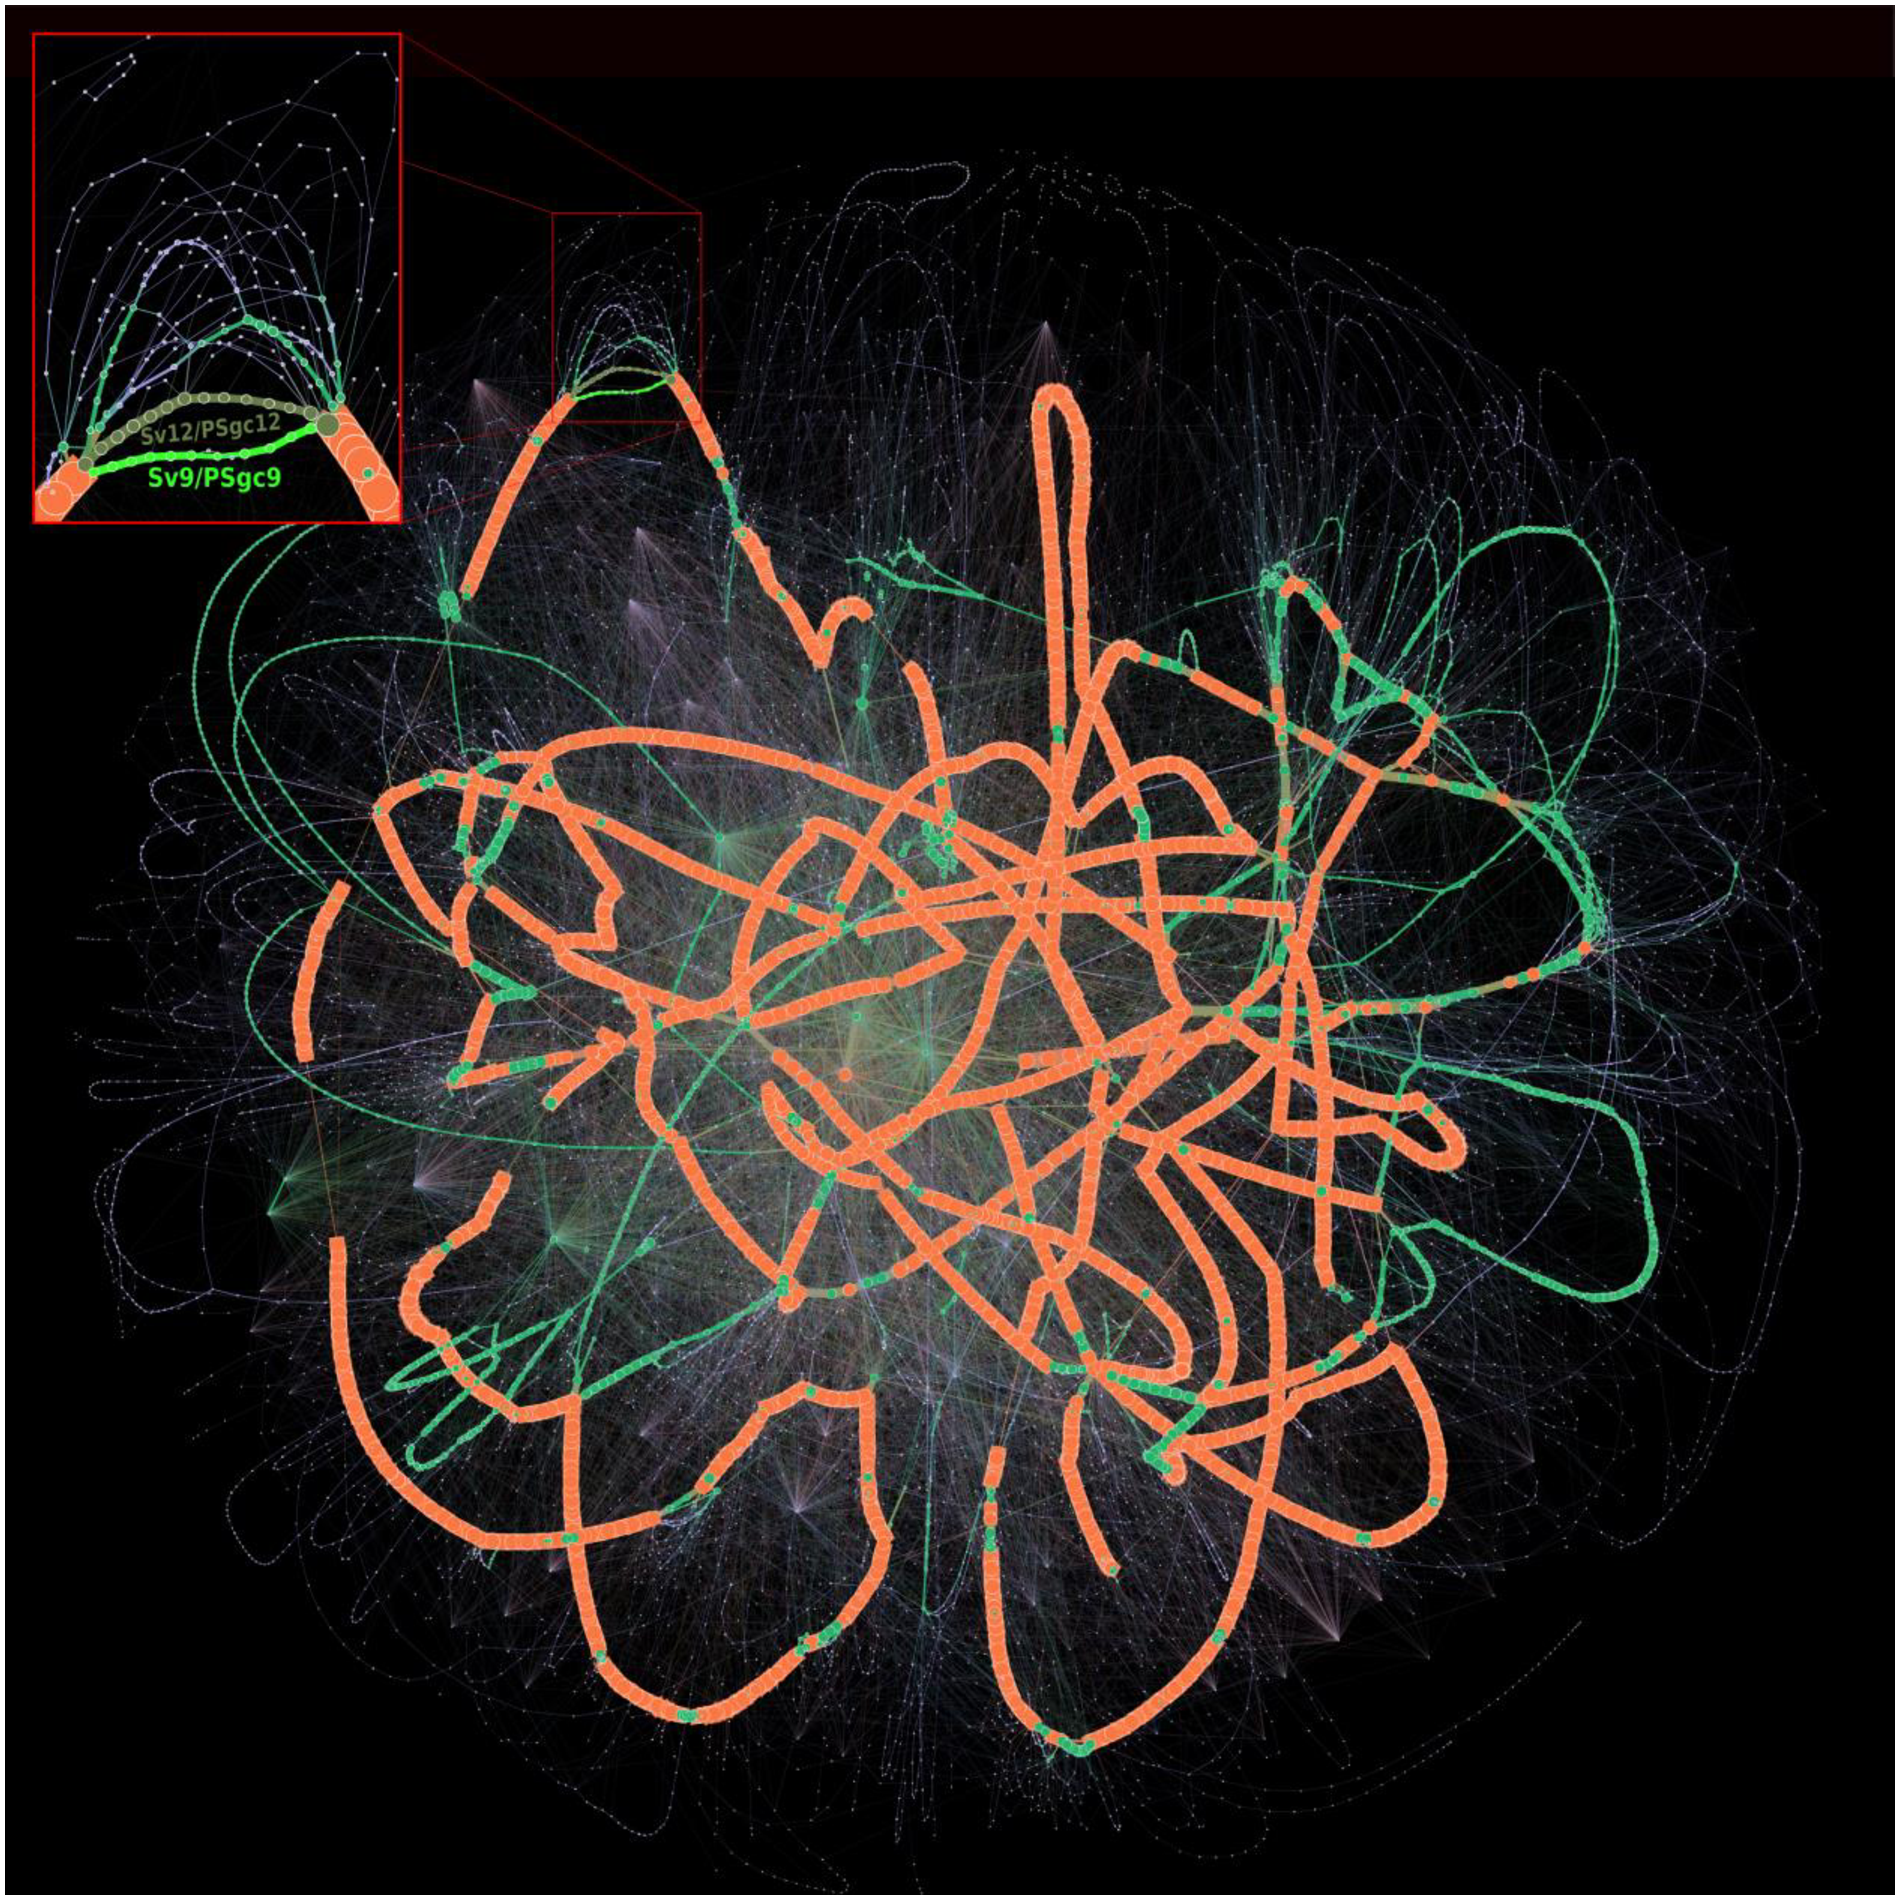
\includegraphics[width=0.6\linewidth]{images/pangenomeAcioneto.png}
    \caption[Graphe de pangénome de \textit{Acinetobacter baumannii}]{\textbf{Graphe de pangénome de \textit{Acinetobacter baumannii}.} Le pangénome est construit avec PPanGGOLiN à partir de 3117 génomes de \textit{A. baumannii}. Les arêtes reliant les familles \textit{persistent}, \textit{shell} et \textit{cloud} sont respectivement colorées en orange, vert et bleu. Les connexions entre familles de gènes appartenant à différentes partitions sont représentées par des couleurs mélangées. Pour améliorer la lisibilité, les familles comptant moins de 20 gènes ne sont pas affichées, bien qu'elles représentent 84,68 \% des n\oe uds (principalement des familles à un seul gène). Un encadré dans le coin supérieur gauche zoome sur une région ramifiée où plusieurs chemins alternatifs \textit{shell} et \textit{cloud} sont présents dans l'espèce. Cette région est impliquée dans la biosynthèse du principal antigène polysaccharidique de \textit{A. baumannii}. Les deux chemins les plus fréquents (Sv12/PSgc12 et Sv9/PSgc9) sont mis en avant en kaki et vert fluorescent.}
    \label{fig:pangenomeBaumannii}
\end{figure}

\section{La méthode PanRGP}

Le logiciel PPanGGOLiN intègre une méthode pour l'identification des régions de plasticité génomique et la prédiction des spots d'insertion, la méthode panRGP \cite{bazin_panrgp_2020}. Cette méthode repose sur l'utilisation du graphe de pangénome partitionné pour ne pas avoir à comparer l'ensemble des génomes (ce qui est déjà fait dans la construction du pangénome) et donc d'être plus efficace que les outils de génomique classique.

\subsection{Identification des régions de plasticité génomique}

Les régions de plasticité génomique sont des objets génomiques : la méthode de prédiction décrite dans la \autoref{fig:panRGP} est appliquée à chaque génome du pangénome, sur lesquels on a projeté les partitions du pangénome.

Pour chaque gène du génome, on calcule un score $s_g$ de manière séquentielle le long des contigs qui est égal au score du gène précédent auquel on applique une pénalité ou une prime en fonction de la partition du gène. Si le gène est \textit{shell} ou \textit{cloud}, on applique une prime correspondant à la somme de 2 constantes, $v$ qui favorise le gène variable et $\epsilon$ pour égaliser les résultats quelque soit le sens de lecture du contig. Si le gène est \textit{persistent}, on applique une pénalité $p$. Pour pénaliser la succession de gènes \textit{persistent}, la pénalité est exponentiellement proportionnelle au nombre ($n$) de gènes \textit{persistent} successifs précédents ($p^n$).   

Si le génome est linéaire, le premier gène de chaque contig aura un score de 0. Dans le cas des séquences circulaires, un premier gène est choisi et un score initial de 0 lui est attribué, puis l’algorithme assigne un score à tous les autres gènes. À la fin du contig, le gène avec un score de 0 est réévalué. Ce nouveau score sert de base pour exécuter une nouvelle boucle de calcul de score qui s'arrête dès qu'un gène obtient un score de 0 ou jusqu’à atteindre le dernier gène du contig.

\begin{figure}[htbp]
    \centering
    \includegraphics[width=0.8\linewidth]{images/panRGP.jpeg}
    \caption[PanRGP : vue d’ensemble de la méthode de détection des RGP]{\textbf{PanRGP : vue d’ensemble de la méthode de détection des RGP.} Les boîtes représentent les gènes codant des protéines : les couleurs orange, vert et bleu correspondent respectivement aux partitions \textit{persistent}, \textit{shell} et \textit{cloud}. Les boîtes en pointillés signalent les gènes appartenant à des familles multigéniques. Dans cet exemple, deux RGP sont détectées : RGP1 avec un score de 5 et RGP2 avec un score de 4. La valeur n associée à chaque gène correspond au nombre de gènes persistants consécutifs en aval. Les valeurs $f(g)$ représentent le résultat d'une fonction utilisée pour calculer le score de chaque gène ($s_g$). Ici, les paramètres par défaut p et v sont fixés respectivement à 3 et 1.}
    \label{fig:panRGP}
\end{figure}

Pour détecter les RGPs, l’algorithme parcourt chaque contig à la recherche du gène ayant le score le plus élevé, à condition qu’il dépasse le seuil $s_{min}$ (fixé par défaut à 4). Ce gène marque la fin initiale de la RGP. Ensuite, les gènes situés en amont sont ajoutés progressivement jusqu’à rencontrer un gène dont le score est nul. La région est alors considérée comme une RGP uniquement si elle contient un nombre de nucléotide supérieur au seuil minimal attendu $l_{min}$ (fixé par défaut à 3 000 bp). Enfin, le score de la RGP est recalculé en repartant du dernier gène détecté, en appliquant la même méthode de calcul que précédemment.

\subsection{Prédiction des spots d'insertion}

Les spots correspondent à des régions où de nombreux éléments se sont insérés au cours de l'évolution, et donc ce sont des régions fortement variables. Aux extrémités de chaque RGP, on sélectionne un nombre \textit{c} de gènes persistants non multigéniques, convertis en familles de gènes pour rendre l’algorithme indépendant de l’orientation.

\newpage

Un graphe $G(V, E)$ est construit, où chaque n\oe ud représente les bordures d’une RGP et chaque arête relie deux n\oe uds ayant des ensembles de familles de gènes similaires. Deux bords sont considérés comme proches si leurs \textit{e} premières familles sont identiques ou si leurs ensembles ordonnés se chevauchent d’au moins \textit{o} familles. Lorsque tous les bords de deux RGPs correspondent, une arête est ajoutée, et les composantes connexes du graphe définissent les spots, auxquels sont associées les RGPs correspondantes.

Les paramètres par défaut sont $c=3$, $e=1$, $o=2$. Chaque spot est évalué selon plusieurs métriques, comme le nombre de RGPs et de familles de gènes. Les RGPs sans $c$ gènes persistants consécutifs ne sont pas prises en compte, car elles sont soit incomplètes (bords de contigs), soit correspondent à des plasmides.

\section{La méthode PanModule}

Dans les génomes, et notamment dans les GIs et les spots, des groupes de gènes sont supposés avoir suivi la même histoire évolutive. Ces ensembles de gènes, cooccurrents et colocalisés, sont appelés des \textbf{modules conservés}. La méthode panModule \cite{bazin_panmodule_2021}, intégrée à PPanGGOLiN, permet de détecter ces modules depuis le graphe de pangénome partitionné. 

\newpage

Tout d'abord, un pangénome est reconstruit à partir des génomes, mais celui-ci intègre, en plus des arêtes de voisinage directes, des arêtes entre les familles séparées dans les génomes d'un espace intergénique inférieur à $t$ gènes. Lorsque $t > 1$, cela équivaut à appliquer une \textbf{fermeture transitive} partielle sur les graphes de génomes, ce qui permet de relier des familles même si leurs gènes ne sont pas directement adjacents. Cette approche est particulièrement utile lorsqu’un module génomique est interrompu par l’insertion d’un gène (comme une séquence d’insertion) ou lorsque des gènes ont été perdus à la suite d’un événement de délétion ou de pseudogénisation.

Les arêtes vont ensuite être filtrées selon deux \textbf{coefficients de similarité de Jaccard} :

\begin{equation}
J(v_i, e_{i,j}) = \frac{w_{e_{i,j}}}{w_{v_i}}, \quad J(v_j, e_{i,j}) = \frac{w_{e_{i,j}}}{w_{v_j}}
\label{eq:jaccard}
\end{equation}

où :
\begin{itemize}
    \item $w_{v_i}$ et $w_{v_j}$ correspondent au nombre de gènes associés aux familles $v_i$ et $v_j$, respectivement.
    \item $w_{e_{i,j}}$ représente le nombre de paires de gènes ayant servi à créer l’arête $e_{i,j}$ entre les nœuds $v_i$ et $v_j$.
\end{itemize}

Un seuil $s$ est défini comme la similarité minimale de Jaccard nécessaire pour considérer une arête comme appartenant à un module. Si les deux coefficients de Jaccard vérifient :

\begin{equation}
J(v_i, e_{i,j}) > s \quad \text{et} \quad J(v_j, e_{i,j}) > s
\end{equation}

alors l’arête est conservée ; sinon, elle est supprimée du graphe. De plus, les n\oe uds correspondant à des familles de gènes présentes dans moins de $m$ génomes sont également retirés.

Après cette phase de filtrage, les \textbf{composantes connexes} du graphe sont extraites à l’aide d’un algorithme de \textbf{parcours en largeur (BFS)} modifié. Une composante est considérée comme un \textbf{module prédit} si elle contient au moins trois n\oe uds appartenant aux familles \textit{shell}, \textit{cloud} ou multigéniques persistantes, selon la classification PPanGGOLiN. En revanche, les modules constitués de \textbf{familles persistantes non multigéniques} ne sont pas pris en compte. Ces familles correspondent généralement à des régions synténiques conservées dans la majorité des génomes étudiés, avec peu ou pas d’événements de réarrangement.

Les modules prédits peuvent ensuite être associés aux autres analyses de PPanGGOLiN, en identifiant sur quelles RGPs et dans quels spots sont retrouvés les modules.

\chapter{Évolution de PPanGGOLiN : présentation de la version 2}

PPanGGOLiN est un outil dont le développement a commencé (sur GitHub) en 2018. Avec plus de 2000 commits\footnote{ajout, suppression ou modification de code validé et marqué dans le système de gestion de version (ici Git)} actuellement, et 7 ans de développement, le code a connu de nombreuses évolutions. De plus, ces modifications sont l'\oe uvre de plusieurs développeurs qui se sont succédés et qui ont collaboré activement au projet.

Le développement de nouvelles méthodes, l'ajout de nouveaux outils, ou encore simplement le débogage devenaient de plus en plus lourds. De plus, dans le cadre de ma thèse, PPanGGOLiN allait être utilisé comme outil et certaines fonctionnalités devaient être améliorées. C'est avec cet objectif en tête que Jean Mainguy (ingénieur au LABGeM), Guillaume Gautreau (chercheur INRAE), Adelme Bazin (ingénieur de recherche), Alexandra Calteau (chercheuse CEA), David Vallenet (directeur de recherche CEA) et moi-même avons développé et proposé en janvier 2024 une version 2 de PPanGGOLiN. Cette nouvelle version contient de nouvelles fonctionnalités pour l'analyse des pangénomes, mais aussi de nombreuses améliorations techniques.

Dans ce chapitre, nous reviendrons sur les changements majeurs apportés dans la version 2 de PPanGGOLiN. D'autres changements plus anecdotiques ne seront pas abordés. Néanmoins, une des améliorations concerne l'écriture des notes de versions qui sont plus détaillées. Toutes les modifications sont alors visibles dans ces notes sur le GitHub de PPanGGOLiN \url{https://github.com/labgem/PPanGGOLiN/releases}.

\section{Nouvelles fonctionnalités et amélioration méthodologique}
\subsection{Developpement de nouvelles méthodes d’analyse}
\subsubsection{Recherche de contexte génomique}

\paragraph{Définition}

Le contexte génomique (\textit{Genomic Context}, GC) désigne l’organisation spécifique des gènes au sein d’un génome. Durant l'évolution, cette organisation va subir des pressions de sélection. Si elle se maintient conservée, on peut postuler que les gènes du GC sont impliqués dans un même processus biologique. C'est pourquoi, la recherche de GCs conservés dans les génomes est utilisée pour prédire la fonction de gènes inconnus en les associant à d'autres dont la fonction est connue. C'est le principe du coupable par association \cite{aravind_guilt_2000}. Rechercher un GC (ou un sous-ensemble de ce dernier) dans les génomes permet ainsi d'identifier des processus biologiques et des dérivés dans les génomes, comme le fait antiSMASH \cite{medema_antismash_2011}, en détectant spécifiquement les clusters de gènes biosynthétiques (BGCs).

\newpage

Une des méthodes de recherche de GC dans les génomes repose sur le voisinage des gènes dans les séquences. On considère des gènes comme fonctionnellement liés s’ils sont régulièrement retrouvés à proximité les uns des autres dans divers génomes, même sans être directement adjacents. Ce type de signal permet de détecter des associations fonctionnelles conservées, même entre des gènes non homologues. 

Cette approche est particulièrement intéressante dans le cadre des graphes de pangénome, comme ceux produits par PPanGGOLiN. Le graphe de pangénome intègre déjà l’information sur le voisinage direct des gènes à travers l’ensemble des génomes étudiés. Cela permet d’extraire efficacement le contexte génomique directement depuis le graphe. De plus, cette approche permet de capturer toute la diversité génomique d’un ensemble d’organismes : non seulement les gènes conservés dans toutes les souches, mais aussi les gènes accessoires, présents uniquement dans certaines d’entre elles. Ainsi, l’extraction du contexte génomique à partir d’un pangénome permet de mieux refléter la diversité biologique réelle tout en accélérant la prédiction fonctionnelle des gènes.

\paragraph{Méthode de recherche de contexte génomique}

L'algorithme de prédiction (\autoref{fig:searchCC}) s’inspire de celui proposé dans panModule \cite{bazin_panmodule_2021}. Cependant, contrairement à ce dernier, qui vise à extraire l’ensemble des contextes génomiques conservés, notre approche se focalise sur l’identification précise des contextes associés à un ensemble de protéines cibles. L’objectif est d’extraire, au sein du pangénome, les familles de gènes conservées dans le contexte de ces protéines.

La première étape consiste à aligner les gènes cibles (\textit{target}) avec les familles de gènes du pangénome. Cet alignement est effectué à l’aide de MMSeqs2 \cite{steinegger_mmseqs2_2017}, avec un seuil de 80 \% d'identité et 80 \% de couverture entre les séquences protéiques des gènes et celles des familles. Les familles correspondant aux séquences alignées sont alors étiquetées comme \textit{target} (représentées en bleu et orange dans la \autoref{fig:searchCC}).

\begin{figure}[htbp]
    \centering
    \includegraphics[width=\linewidth]{images/searchCC.png}
    \caption[Méthode de recherche du contexte génomique dans un graphe de pangénome]{\textbf{Méthode de recherche du contexte génomique dans un graphe de pangénome.}}
    \label{fig:searchCC}
\end{figure}

\newpage
À partir de ces familles \textit{target}, nous reconstruisons un sous-graphe du pangénome. Ce sous-graphe intègre non seulement les arêtes de voisinage direct, mais aussi des arêtes de transitivité reliant des familles situées à une distance $t$. Ainsi, l’algorithme capture non seulement les relations directes, mais aussi celles entre familles avoisinantes. Par exemple, dans la \autoref{fig:searchCC}, avec $t=1$, des arêtes de transitivité sont créées entre le gène bleu et les gènes vert et noir, ainsi qu'entre le gène violet et les gènes rouge et gris.

Pour limiter la taille du sous-graphe, un paramètre \textit{window} est introduit. Il contrôle le nombre de gènes adjacents — de part et d'autre de la \textit{target} — pris en compte pour la création des arêtes de transitivité.

Le sous-graphe obtenu forme alors une composante connexe intégrant l’ensemble des relations de voisinage jusqu’à la distance $t$. Un filtre de Jaccard (cf. \autoref{eq:jaccard}) est ensuite appliqué pour conserver uniquement les arêtes les plus pertinentes.

Enfin, nous extrayons toutes les composantes connexes contenant au moins une famille \textit{target}, représentant ainsi les contextes génomiques conservés autour des protéines cibles.

\subsubsection{Metadonnées}

Dans le cadre de l'ajout de nouvelles fonctionnalités à PPanGGOLiN, une première avancée que j'ai développée concerne l'ajout de \textbf{métadonnées} à l'ensemble des éléments du pangénome, incluant les gènes, contigs, génomes, familles, arêtes, RGPs, spots et modules. Le format attendu des métadonnées est particulièrement flexible, l'utilisateur fournit un fichier tabulé, ne nécessitant au minimum que l'identifiant de l'objet concerné dans le pangénome.  L’utilisateur peut ainsi associer des métadonnées de tout type, sans restriction de format. De plus, chaque métadonnée est liée à une source spécifique, ce qui permet à un même objet d’en contenir plusieurs, issues de différentes sources d’annotation. Pour assurer une gestion optimisée et performante, ces métadonnées sont directement enregistrées dans le fichier HDF5 du pangénome. Bien qu'elles ne soient pas directement exploitées pour l'analyse du pangénome, elles sont intégrées aux sorties générées par PPanGGOLiN afin de faciliter l'interprétation et l'exploration des résultats.

\subsubsection{Projection}

Pour faciliter l'exploration des résultats, une \textbf{nouvelle sortie de visualisation des données} a été développée en collaboration avec Jean Mainguy. Celle-ci permet de générer, pour chaque génome, un fichier JSON compatible avec Proksee \cite{grant_proksee_2023}. Grâce à cette fonctionnalité, il est désormais possible de visualiser un génome, sous forme circulaire (\autoref{fig:projection}), où les éléments du pangénome ont été intégrés, notamment les parties persistantes et variables, ainsi que les RGPs, spots et modules. Proksee permet également de lancer des analyses supplémentaires sur les génomes, comme CARD \cite{alcock_card_2023} pour annoter les gènes de résistance aux antibiotiques, CRISPRCasFinder \cite{couvin_crisprcasfinder_2018} pour la prédiction des systèmes CRISPR-Cas, ou encore Phigaro \cite{starikova_phigaro_2020} qui permet d'identifier les régions de prophages. 

\newpage
L'intégration de cette nouvelle sortie est d'autant plus intéressante dans une autre nouvelle fonctionnalité de PPanGGOLiN : la \textbf{projection} des résultats du pangénome sur un génome externe. En effet, il est désormais possible de comparer un nouveau génome au pangénome déjà calculé. Pour cela, les gènes du génome externe sont alignés aux séquences référentes des familles de gènes en utilisant MMSeqs2 \cite{steinegger_mmseqs2_2017}. Les gènes dont l'alignement dépasse un seuil défini d'identité et de couverture sont alors associés à une famille existante, tandis que les autres gènes forment chacun une nouvelle famille (singleton) attribuée à la partition du \textit{cloud}. Ainsi, l’ensemble des gènes du génome externe se voit assigner une partition, ce qui permet d’appliquer les algorithmes de prédiction des RGPs et d’associer les spots et les modules au génome étudié.

Enfin, cette fonctionnalité de projection prend également en compte les métadonnées, assurant ainsi la transmission des informations du pangénome aux gènes du génome externe. Cette intégration renforce la cohérence des analyses en permettant d’exploiter les annotations des utilisateurs pour une meilleure interprétation des résultats.

\begin{figure}[htbp]
    \centering
    \includegraphics[width=\linewidth]{images/projection.png}
    \caption[Principe de fonctionnement de la méthode de projection]{\textbf{Principe de fonctionnement de la méthode de projection.} Le génome sur lequel le pangénome est projeté, est un génome de la même espèce que ceux qui ont servi à construire le pangénome. Sur la droite, un exemple de sortie disponible dans PPanGGOLiN et généré dans les projections, le Proksee \cite{grant_proksee_2023} d'un génome de \textit{A. baumannii} où les résultats du pangénome ont été projeté.}
    \label{fig:projection}
\end{figure}

\subsubsection{Analyse comparée des RGPs}

Une nouvelle fonctionnalité a été intégrée à PPanGGOLiN pour permettre l’analyse comparative des RGPs entre plusieurs génomes d’un même pangénome. Désormais, il est possible de regrouper (clusteriser) les RGPs similaires  (\autoref{fig:rgpcluster_met}). Deux RGPs sont considérés comme partageant un contenu commun si leurs gènes appartiennent aux mêmes familles de gènes. À partir de cette définition, un score de correspondance du répertoire génique (\textit{Gene Repertoire Relatedness}, GRR) est calculé, soit sur la RGP la plus petite, soit sur la plus grande :

\begin{equation}
\begin{split}
GRR_{min} = \frac{\text{nombre de gènes partagés}}{\text{nombre de gènes de la plus petite RGP}} \\
GRR_{max} = \frac{\text{nombre de gènes partagés}}{\text{nombre de gènes de la plus grande RGP}}
\end{split}
\end{equation}

Le processus de clustering repose sur une modélisation par graphe. Chaque RGP est représentée sous forme d’un n\oe ud, et une arête est ajoutée entre deux n\oe uds si leur GRR dépasse un seuil défini (0,8 par défaut). Ainsi, chaque composante connexe du graphe correspond à un ensemble de RGPs partageant un même répertoire génique.

Les résultats du clustering sont disponibles soit sous forme d'un fichier tabulé récapitulant les regroupements obtenus, soit dans des outils de visualisation de graphe comme Gephi \cite{bastian_gephi_2009} ou Cytoscape \cite{shannon_cytoscape_2003}.

L’intégration des métadonnées prend de nouveau tout son sens. Il est possible d’annoter et de colorer les graphes en fonction des métadonnées associées aux gènes du pangénome, ce qui facilite l’interprétation biologique des clusters obtenus. Un exemple d’application est illustré en \autoref{fig:rgpcluster_app}, où le clustering des RGPs du pangénome de \textit{A. baumannii} a été réalisé. Les gènes ont été annotés avec CARD \cite{alcock_card_2023} pour identifier les éléments liés à la résistance aux antibiotiques. Deux clusters ont été extraits en guise d'exemple. Le cluster de gauche correspond à un ensemble de RGPs localisés dans un même spot (13). Parmi eux, trois RGPs sont associées à des \textbf{gènes de résistance aux antibiotiques }(n\oe uds en forme de triangle). Le cluster de droite regroupe des RGPs répartis sur huit spots distincts, révélant ainsi une mobilité plus variée dans les génomes. Contrairement au premier cluster, ces RGPs ne sont pas directement associées à des gènes de résistance. Cependant, d’autres métadonnées, par exemple des annotations métaboliques, pourraient être intégrées pour identifier des fonctions communes entre ces spots.

\begin{figure}[htbp]
    \centering
    \subfloat[Méthode de clusterisation des RGPs]{\includegraphics[width=\linewidth]{images/clusterRGPs.png}
    \label{fig:rgpcluster_met}}
    \hfill
    \subfloat[Application du clustering des RGPs sur le pangénome de \textit{A. baumannii} avec des métadonnées de résistance aux anitbiotiques (AMR)]{\includegraphics[width=\linewidth]{images/rgpclusterappli.png}
    \label{fig:rgpcluster_app}}
    \caption[Clustering des RGPs]{\textbf{Clustering des RGPs.}}
    \label{fig:rgpcluster}
\end{figure}

\subsection{Amélioration des procédures d'analyses}

\subsubsection{Lecture des fichiers d'annotation}

PPanGGOLiN permet la construction d'un graphe de pangénome à partir de séquences nucléiques et de génomes préalablement annotés. Les fichiers de génomes annotés (aux formats GFF ou GBFF) contiennent déjà les gènes ainsi que leurs coordonnées (contig, position, brin \dots). Ces fichiers peuvent également inclure des informations sur la fonction des gènes, des métadonnées relatives aux génomes et aux contigs, ainsi que la séquence des gènes ou des contigs eux-mêmes. Jusqu'à récemment, une partie de ces informations était ignorée par PPanGGOLiN. Désormais, elles sont lues et stockées dans le fichier de pangénome sous forme de métadonnées.

En nous intéressant à l'annotation fonctionnelle du pangénome, nous avons observé des divergences entre les séquences issues des fichiers d'annotation et celles correspondant aux gènes et aux familles de gènes. Nous avons notamment constaté que certaines coordonnées de gènes présentaient une complexité particulière et correspondaient à des événements biologiques spécifiques, tels que des décalages du cadre de lecture (\textit{frameshift}). Un ensemble de cas présentant des coordonnées atypiques a ainsi été identifié et est désormais correctement pris en charge dans PPanGGOLiN.

Ces améliorations ont conduit à une meilleure construction des familles de gènes, en corrigeant des séquences auparavant incorrectement tronquées ou décalées. Par ailleurs, elles ont permis d'améliorer la réécriture des séquences dans les fichiers de sortie, notamment ceux destinés à Proksee \cite{grant_proksee_2023}, et, par conséquent, la qualité des annotations fournies par les outils intégrés à cette plateforme.

\newpage

\subsubsection{Exécution de PPanGGOLiN via un fichier de configuration}

PPanGGOLiN intègre désormais la possibilité de générer un fichier de configuration. Ce fichier contient l’ensemble des commandes de PPanGGOLiN pouvant être exécutées ainsi que les paramètres spécifiques à chaque commande et les  globaux. A partir de ce fichier, PPanGGOLiN peut lancer une analyse \textit{de novo} sans préciser les paramètres de la ligne de commande. Ce fichier offre ainsi une alternative plus souple et organisée à l’exécution classique en ligne de commande. Il présente aussi plusieurs avantages.
(\textit{i}) Une exécution entièrement paramétrable des workflows. Jusqu’à présent, l’exécution de PPanGGOLiN dans un workflow reposait sur un nombre restreint de paramètres en ligne de commande. Cette limitation visait à éviter une surcharge des lignes de commande ainsi que d’éventuels conflits de nommage entre paramètres. Grâce aux fichiers de configuration, il devient possible de paramétrer entièrement un workflow, en définissant de manière explicite toutes les options requises. 
(\textit{ii}) Une intégration facilitée dans les pipelines d’analyse. L’utilisation de fichiers de configuration simplifie considérablement l’intégration de PPanGGOLiN dans des pipelines d’analyse. En effet, l’exécution d’outils en ligne de commande au sein de pipelines automatisés (souvent via des scripts Bash) peut poser plusieurs difficultés, telles que : une mauvaise interprétation des types de paramètres (par exemple, un entier lu comme une chaîne de caractères), des erreurs dans la gestion des chemins de fichiers, des conflits entre options spécifiques. L’emploi d’un fichier de configuration permet d’éliminer ces problèmes en standardisant et sécurisant la transmission des paramètres. Cette approche a notamment été adoptée lors de l’intégration de PPanGGOLiN dans MicroScope \cite{vallenet_microscope_2020}.

L’ajout des fichiers de configuration s’inscrit également dans les principes FAIR\footnote{Les principes FAIR visent à garantir que les données et les logiciels scientifiques soient faciles à retrouver (Findable), accessibles (Accessible), interopérables (Interoperable) et réutilisables (Reusable). Bien que ces principes aient été initialement conçus pour les données et le \textit{Big Data}, ils s’appliquent également aux outils bioinformatiques.}. En particulier, ils renforcent la reproductibilité des analyses. PPanGGOLiN permet ainsi de générer, à partir d’un pangénome, un fichier de configuration contenant toutes les options ayant permis sa construction. Cela garantit que, pour un même jeu de données, les analyses restent strictement reproductibles, favorisant ainsi une science plus ouverte et plus éthique. Cette avancée est particulièrement bénéfique dans un contexte de publication scientifique, où la transparence et la reproductibilité des analyses sont essentielles.

\newpage

\section{Optimisation technique}

Au-delà de l’ajout de nouvelles fonctionnalités, la version 2 de PPanGGOLiN a bénéficié de nombreuses améliorations visant à optimiser son efficacité, son ergonomie et sa maintenabilité. Parmi celles-ci, les optimisations techniques ont joué un rôle clé en réduisant la taille des fichiers générés, les temps de lecture ainsi que la mémoire utilisée.

\subsection{Amélioration de l'efficacité de PPanGGOLiN}

L’une des améliorations concerne l’optimisation du processus d’annotation des génomes. À cette fin, l’exécution de Prodigal \cite{hyatt_prodigal_2010} a été remplacée par l’intégration de Pyrodigal \cite{larralde_pyrodigal_2022}. Ce changement présente deux avantages principaux. 
Premièrement, la réduction des entrées/sorties (I/O) et l'amélioration de la gestion de la mémoire. Contrairement à l'exécution de Prodigal, qui nécessitait de générer des fichiers intermédiaires contenant les résultats d’annotation, Pyrodigal retourne directement les annotations sous forme d’objets Python utilisables par PPanGGOLiN. Cette approche permet de ne pas avoir à écrire et lire des fichiers intermédiaires pour chaque génome, réduisant ainsi l’empreinte mémoire et améliorant l’efficacité des opérations d’I/O. Deuxièmement, Pyrodigal intègre plusieurs améliorations au moteur de Prodigal, notamment une optimisation du calcul du score de connexion. Ce score est utilisé pour évaluer la probabilité d’une transition entre deux codons en fonction de divers critères (cadre de lecture, type de codon – initiation ou stop –, orientation du brin\dots). Comme l’a souligné Larralde \cite{larralde_pyrodigal_2022}, le calcul du score de connexion sur de longues séquences peut être coûteux en temps de calcul. Pyrodigal améliore ce processus en implémentant un filtrage heuristique, qui permet d’ignorer les connexions clairement invalides dès le départ. De plus, Pyrodigal exploite les fonctionnalités SIMD (Single Instruction, Multiple Data) des CPU modernes pour traiter plusieurs n\oe uds de calcul simultanément. Cela permet de traiter 8 n\oe uds avec les fonctionnalités NEON et SSE2, et 16 n\oe uds avec AVX2 (\autoref{fig:pyrodigal}). Ces optimisations réduisent le temps de calcul et améliorent significativement l’efficacité globale de la prédiction des gènes dans PPanGGOLiN.

\begin{figure}[htbp]
    \centering
    \includegraphics[width=0.8\linewidth]{images/pyrodigal.png}
    \caption[Évaluation des performances de calcul des scores de connexions]{\textbf{Évaluation des performances de calcul des scores de connexion.} L'évaluation est réalisé avec différents backends SIMD pour le filtre heuristique (SSE2 ou AVX2), avec un backend générique (\textit{Generic}) ou sans activer le filtre (\textit{None}). Chaque séquence a été traitée 10 fois sur un processeur \textit{i7-10710U} à 1,10 GHz. Extrait de \cite{larralde_pyrodigal_2022}}
    \label{fig:pyrodigal}
\end{figure}

Toujours dans l'objectif d'amélioration de l’efficacité de PPanGGOLiN, les fonctions de lecture ont été revues, afin de réduire le temps de chargement des données et l’utilisation de la mémoire. 
Pour atteindre cet objectif, plusieurs modifications ont été apportées à la manière dont les objets du pangénome sont interconnectés, afin de limiter le chargement de données inutiles. Dans PPanGGOLiN, la structure hiérarchique des objets implique, par exemple qu’un gène appartient à un contig, lequel est lui-même rattaché à un génome. Or, dans certaines commandes, le chargement des gènes entraînait systématiquement celui des contigs et des génomes, augmentant ainsi le temps d’exécution. Pour pallier ce problème, nous avons réorganisé ces dépendances et réécrit plusieurs fonctions de lecture afin de rendre l’accès aux données plus sélectif et plus efficace.

L’une des améliorations les plus significatives concerne la lecture des spots. Une réécriture de cette fonction a permis une réduction drastique du temps de lecture. Sur un pangénome de 3 083 génomes de \textit{E. coli}, le temps de lecture de 2 036 spots est passé de 25 minutes (dans un temps total de lecture du pangénome de 36 minutes) à seulement 3,5 secondes (pour un temps total réduit à 9 minutes et 38 secondes)\footnote{Cette amélioration est particulièrement visible sur les pangénomes de grande taille contenant un nombre important de spots, ce qui explique pourquoi le problème n’avait pas été détecté auparavant.}.

Dans cette même optique, des améliorations ont également été apportées à l’écriture des séquences (nucléotidiques et protéiques). Dans les versions précédentes de PPanGGOLiN, pour faciliter le filtrage des séquences demandées par l’utilisateur, l’ensemble du pangénome et de ses objets était chargé en mémoire, ce qui entraînait une consommation importante de ressources. Désormais, les séquences sont directement extraites du fichier HDF5, évitant ainsi la recréation systématique des objets du pangénome et réduisant significativement l’utilisation de la mémoire.

Avec l’augmentation continue du nombre de génomes disponibles, les pangénomes générés par PPanGGOLiN sont devenus de plus en plus volumineux. Malgré une structure de stockage compacte, reposant sur le package PyTable \cite{team_pytables_2002}, la taille des fichiers HDF5 a considérablement augmenté, en raison du nombre croissant de génomes et des nouvelles fonctionnalités enrichissant les données stockées.
Pour remédier à ce problème, l’architecture interne du fichier HDF5 a été revue afin d’éliminer les redondances, en particulier dans l’annotation des gènes et de leur séquence. En effet, entre différents génomes, les gènes peuvent partager des caractéristiques communes telles que leur position, leurs coordonnées ou encore leur orientation sur le brin. Or, ces informations étaient systématiquement dupliquées dans l’ancienne structure. Afin de réduire cette redondance, une table de référence a été mise en place pour centraliser ces informations et leur attribuer un identifiant unique, à la manière d’une base de données relationnelle. Chaque gène peut ainsi être associé à son annotation optimisée, sans nécessiter la répétition de ses caractéristiques dans l’ensemble du pangénome.
Cette optimisation a permis une réduction significative de la taille des fichiers HDF5. Comme illustré en \autoref{fig:ppanggoSize}, la taille des pangénomes a été divisée par 3,5 pour un ensemble de 1 000 génomes, et par 6,5 pour un pangénome de 2 500 génomes.
Au-delà du gain en espace de stockage, cette amélioration contribue également à l’accélération des temps de lecture. En effet, elle participe à la lecture non systématique des informations liées aux gènes lors du chargement du pangénome, ce qui allège le processus et améliore les performances globales de l’outil.

\begin{figure}
    \centering
    \includegraphics[width=.8\linewidth]{images/benchPPanGGO.png}
    \caption[Taille des fichiers de pangénome entre la version 1 et 2 de PPanGGOLiN]{\textbf{Comparaison des tailles des fichiers de pangénome entre la version 1 et 2 de PPanGGOLiN.}}
    \label{fig:ppanggoSize}
\end{figure}

Ces optimisations rendent PPanGGOLiN plus performant, plus rapide et plus adapté aux analyses pangénomiques de grande échelle, tout en maintenant une gestion efficace des ressources.

\subsection{Optimisation du code : lisibilité, maintenance, tests et processus de mise à jour}

En tant que logiciel open source, le code de PPanGGOLiN est accessible à tous, conformément aux principes de la science ouverte. Ce choix présente plusieurs avantages : il permet à la communauté d’utilisateurs de signaler d’éventuels comportements inattendus (problèmes de performance, bugs, \textit{etc}.), mais aussi de contribuer directement à l’amélioration du logiciel en proposant des corrections ou des optimisations.
Afin d’assurer la pérennité et la maintenabilité du projet, nous avons entrepris une révision complète du code, avec pour objectif principal de le rendre plus lisible, homogène et facile à maintenir pour les développeurs actuels et futurs.

\subsubsection{Mise en place de bonnes pratiques de développement}

La première étape du reformatage a consisté à aligner PPanGGOLiN avec les versions maintenues et corrigées de Python. Les packages les plus utilisés suivent également cette logique. En mettant à jour le code pour être compatible avec les versions récentes de Python, nous bénéficions des dernières mises à jour des packages, ainsi que des optimisations et corrections apportées par le langage lui-même. Ainsi, nous sommes passés de Python 3.8 à Python 3.12.

Pour améliorer la lisibilité et garantir une cohérence au sein du code, nous avons introduit un ensemble de règles et de processus applicables pour tous les développeurs. La première étape a été l’adoption des bonnes pratiques de codage en Python, en suivant les recommandations des PEP (\textit{Python Enhancement Proposals}).
L’application de ces directives présente plusieurs bénéfices. Premièrement, le code est plus structuré et lisible. Par exemple, les conventions de nommage permettent d’identifier rapidement la nature des variables et objets :

\begin{itemize}
    \item Nom des classes en CamelCase (\textit{e.g.} GeneCluster)
    \item Constantes en majuscules (\textit{e.g.} MAX\textunderscore ITERATIONS)
    \item Fonctions et méthodes en snake\textunderscore case (\textit{e.g.} compute\textunderscore similarity\textunderscore score)
\end{itemize}

Cette homogénéité facilite la lecture et la compréhension du code par tous les contributeurs. Deuxièmement, les règles PEP permettent de mettre en place des micro-optimisations pour de meilleures performances. Par exemple, en privilégiant l’utilisation de générateurs plutôt que des listes temporaires, ce qui permet d’optimiser l’utilisation de la mémoire.

Afin de faciliter l’application de ces règles et d’assurer leur respect de manière systématique, nous avons intégré le package python Black (\url{https://github.com/psf/black}) pour le formatage automatique du code. Lors de chaque mise à jour du code sur GitHub, Black est exécuté automatiquement pour reformater le code selon les standards des PEP. Cette automatisation garantit une cohérence stylistique, réduit la charge de travail des développeurs et simplifie la gestion des contributions extérieures.

Grâce à ces améliorations, le code de PPanGGOLiN devient plus clair, plus performant et plus facile à maintenir, assurant ainsi une plus grande longévité au projet et une meilleure collaboration au sein de la communauté open source.

\subsubsection{Maintenance et test du code}

PPanGGOLiN est avant tout un projet de recherche scientifique, ce qui implique des mises à jour fréquentes pour intégrer de nouvelles fonctionnalités et améliorer ses performances. Toutefois, ces modifications peuvent introduire des bogues susceptibles d’altérer la fiabilité des analyses. Afin de garantir la stabilité et la robustesse du logiciel, nous avons grandement amélioré la stratégie de tests automatisés, couvrant différents niveaux de validation.

\paragraph{Tests unitaires : validation des fonctionnalités élémentaires}

Les premiers tests mis en place sont des tests unitaires, qui permettent de vérifier le comportement individuel des fonctions. Ces tests s’assurent que chaque fonction produit bien le résultat attendu, et qu’elle génère les erreurs appropriées en cas d’entrée invalide. Actuellement, l'ensemble des classes sont testées et ainsi qu'une grande partie des fonctions.

\newpage

\paragraph{Tests d’intégration : validation des interactions entre fonctions}

Nous avons également mis en place des tests d'intégration, visant à évaluer le comportement global du logiciel lorsque plusieurs fonctions interagissent. En effet, une fonction peut répondre comme attendu de manière isolée tout en produisant des comportements imprévus lorsqu'elle est combinée à d'autres modules. Ces tests permettent donc de garantir la cohérence de l'ensemble du programme. Cependant, leur mise en \oe uvre reste complexe en raison des nombreuses interactions entre les fonctions dans PPanGGOLiN, ce qui limite la couverture de cette approche à une partie restreinte du code.

\paragraph{Tests fonctionnels : validation du comportement des commandes}

Enfin, nous avons introduit des tests fonctionnels, qui vérifient le comportement des commandes complètes. Pour cela, des fichiers de résultats de référence ont été préchargés, permettant de comparer automatiquement les nouvelles sorties avec les résultats attendus. Cette approche garantit que les évolutions du code n’altèrent pas l’exactitude des analyses produites par PPanGGOLiN. Toutes les commandes de PPanGGOLiN sont testées en prenant en compte tous les paramètres.


Lors d'une mise à jour du code, un workflow automatique est exécuté et permet de vérifier que le code est bien fonctionnel. Grâce à cette infrastructure de tests, le code est désormais plus robuste, limitant ainsi l’introduction de bogues imprévus et assurant la fiabilité des résultats scientifiques générés par le logiciel.

\subsubsection{Amélioration de l'expérience utilisateur}

PPanGGOLiN est un logiciel conçu pour les microbiologistes, dont l’expertise principale n’est pas nécessairement l’informatique. Il est donc essentiel de garantir une expérience utilisateur fluide, en facilitant aussi bien l’installation que l’utilisation du logiciel.

Un premier effort a été porté sur la réécriture complète de la documentation, afin de la rendre plus claire, plus structurée et mieux adaptée aux besoins des utilisateurs. Désormais, elle comprend :

\begin{itemize}
    \item Une section d’installation détaillant plusieurs méthodes adaptées à différents environnements,
    \item Un guide de prise en main rapide pour permettre aux utilisateurs d’exécuter rapidement PPanGGOLiN et ses principaux workflows,
    \item Des sections approfondies décrivant en détail chaque commande et analyse réalisable,
    \item Un guide dédié aux développeurs, recensant les bonnes pratiques et les processus de développement spécifiques à PPanGGOLiN.
\end{itemize}

De plus, la documentation est maintenant disponible sur ReadTheDocs, ce qui la rend plus accessible, mieux référencée et conforme aux principes FAIR.

\newpage

Un autre aspect clé de l’amélioration de l’expérience utilisateur concerne la gestion des erreurs. Afin de rendre les messages d’erreur plus explicites et plus informatifs, nous avons entrepris une révision complète de leur génération.
Les erreurs liées à une mauvaise utilisation par l’utilisateur sont maintenant décrites de manière plus claire et pédagogique. Les erreurs techniques, destinées aux développeurs, sont quant à elles plus précises, facilitant ainsi l’identification rapide de l’origine du problème. De plus, un plus large éventail de messages a été introduit pour couvrir davantage de cas d’erreur et améliorer la gestion des exceptions.


Grâce à ces améliorations, PPanGGOLiN devient plus intuitif pour les microbiologistes et plus facile à maintenir pour les développeurs, garantissant ainsi une expérience utilisateur optimisée.




\chapter{Application à l'étude de la dégradation du D-Apiose}

Le D-Apiose est un sucre de type pentose, principalement retrouvé dans la paroi cellulaire des plantes vasculaires, mais également présent en tant que métabolite secondaire \cite{picmanova_apiose_2016}. Chez les bactéries, plusieurs voies de dégradation du D-Apiose ont été identifiées \cite{carter_functional_2018}. Parmi celles-ci, la voie de la transcétolase non oxydante (\autoref{fig:apiosePathway}) constitue un mécanisme clé. Cette voie permet la conversion du D-Apiose en D-xylulose 5-phosphate, un métabolite intermédiaire central impliqué dans de nombreuses voies métaboliques essentielles. La voie de la transcétolase non oxydante a été détectée chez diverses bactéries du sol, notamment \textit{Actinobacillus succinogenes} et \textit{Bacteroides vulgatus}, ainsi que chez plusieurs espèces du genre \textit{Pectobacterium}.

En collaboration avec Guilhem Royer (AP-HP) et Erick Denamur (IAME), le LABGeM a identifié une voie alternative chez \textit{Escherichia coli}, où l'isomérase de la première réaction est remplacée par une succession de deux oxydoréductases. Cette voie a été initialement identifiée spécifiquement dans les \textit{Sequence Types} (ST) 131 et 14 de \textit{E. coli}, des souches pathogènes connues pour leur multirésistance aux antibiotiques et leur implication dans les bactériémies\footnote{Infection bactérienne présente dans le sang.} \cite{schembri_molecular_2015,de_korne-elenbaas_putative_2023}. Ces souches colonisent principalement le tube digestif, où la capacité à dégrader le D-Apiose pourrait conférer un avantage sélectif, améliorant ainsi le \textit{fitness} de ces pathogènes.

Dans ce cadre, j’ai contribué au projet en explorant les pangénomes afin d’identifier le contexte génomique associé à la fois à la voie classique (transcétolase non oxydante) et à la voie alternative de dégradation du D-Apiose.

\begin{figure}[htbp]
    \centering
    \includegraphics[width=0.75\linewidth]{images/ApiosePathway.png}
    \caption[Voie de dégradation du D-Apiose par la transcétolase non oxydante]{\textbf{Voie de dégradation du D-Apiose par la transcétolase non oxydante.} (a) Métabolites et réactions de la voie. La première réaction (en vert) correspond à l'isomérisation du D-Apiose en D-Apulose, catalysée par la D-Apiose isomérase. Le D-Apulose est ensuite phosphorylé en D-Apulose 4-phosphate (en rouge) par l’action d’une kinase. Enfin, la dernière transformation (en bleu) est catalysée par la transcétolase, qui permet la production du D-xylulose 5-phosphate. (b) Contexte génomique de la voie de dégradation chez cinq espèces bactériennes. Les gènes impliqués sont représentés par des flèches colorées, dont la couleur correspond à l’enzyme codée. Les gènes gris codent des SBP (protéines de liaison spécifiques) impliqués dans la reconnaissance du D-Apiose, tandis que les gènes noirs codent des composants d’un système de transport ABC. Extrait de \cite{carter_functional_2018}.}
    \label{fig:apiosePathway}
\end{figure}

\section{Recherche du contexte génomique chez les procaryotes}

Nous avons commencé par rechercher la voie de dégradation du D-Apiose, à la fois sous sa forme classique (transcétolase non oxydante) et sous sa forme alternative, dans les espèces procaryotes. Pour cela, nous avons analysé le contexte génomique associé aux six protéines clés impliquées dans ces voies. Ces protéines incluent : 3 enzymes communes aux deux voies, les deux sous-unités de la transcétolase et la kinase; une enzyme spécifique à la voie classique l'isomérase; 2 enzymes spécifiques à la voie alternative, les oxydoréductases.

L’analyse du contexte génomique a été réalisée sur un ensemble de 1 429 pangénomes d’espèces, générés à l’aide de l’outil PPanGGOLiN\footnote{Les pangénomes ont été élaborés dans le cadre du projet PanGBank, visant à constituer une base de données de pangénomes d’espèces.}. Ces pangénomes ont été construits à partir de 152 717 génomes issus de la base de données RefSeq \cite{pruitt_ncbi_2007}, en utilisant la taxonomie GTDB \cite{parks_standardized_2018} pour organiser les génomes par espèce (version RefSeq/GTDB : 220).

\newpage

Le GC de dégradation du D-Apiose a été identifié dans 125 espèces, réparties sur 43 genres, 17 familles, 15 ordres, 7 classes et 4 phylums (\autoref{fig:PhyloTreeApiose}). Parmi ces familles, les \textbf{Enterobacteriaceae} sont les plus représentées (66 espèces), suivies des \textbf{Rhizobiaceae} (23 espèces) et des \textbf{Pseudomonadaceae} (12 espèces). Cette répartition suggère que la voie de dégradation du D-Apiose est relativement fréquente chez les bactéries.
L’analyse de la distribution des données au sein des partitions du pangénome révèle que cette voie est principalement associée à un contexte \textit{persistent}, avec 28 genres sur 43 présentant une majorité de familles classées dans cette même partition.

Parmi les contextes identifiés, seules 7 espèces présentent la voie classique de dégradation du D-Apiose. Six d’entre elles appartiennent au genre \textit{Pectobacterium} : \textit{P. atrosepticum}, \textit{P. brasiliense}, \textit{P. parmentieri}, \textit{P. carotovorum}, \textit{P. versatile} et \textit{P. polare}. La septième espèce, \textit{Novosphingobium capsulatum}, appartient à la famille des \textit{Sphingomonadaceae} et est représentée en bleu-vert clair sur la \autoref{fig:PhyloTreeApiose}. Contrairement aux espèces du genre \textit{Pectobacterium}, où le contexte génomique est retrouvé dans la partition \textit{persistent}, celui de \textit{N. capsulatum} se situe dans la partition \textit{shell}, ce qui pourrait suggérer un transfert horizontal de gènes (HGT) entre ces espèces.

Par ailleurs, 3 espèces possèdent une version hybride entre la voie classique et la voie alternative, caractérisée par la présence simultanée de l’isomérase et des 2 oxydoréductases. Deux d’entre elles appartiennent à la famille des \textit{Sphingomonadaceae}, à savoir \textit{Sphingobium yanoikuyae} et \textit{Sphingomonas koreensis}, tandis que la troisième, \textit{Klebsiella aerogenes}, appartient aux \textit{Enterobacteriaceae}. La présence de voies hybrides dans certaines espèces pourrait refléter une adaptation évolutive conférant une plus grande flexibilité métabolique en fonction des conditions environnementales.

\newpage

Enfin, des contextes partiels ont été détectés dans 13 espèces. Dix d’entre elles appartiennent à la famille des \textit{Enterobacteriaceae}, incluant \textit{Salmonella diarizonae}, \textit{Atlantibacter hermannii}, \textit{Yersinia enterocolitica}, \textit{Leclercia adecarboxylata}, \textit{Citrobacter youngae}, \textit{Yersinia bercovieri}, \textit{Kosakonia radicincitans}, \textit{Yersinia mollaretii}, \textit{Yersinia massiliensis} et \textit{Yersinia intermedia}. Deux autres espèces, \textit{Paracidovorax avenae} et \textit{Paracidovorax citrulli}, appartiennent à la famille des \textit{Burkholderiaceae}, tandis que \textit{Clostridioides difficile} représente la famille des \textit{Peptostreptococcaceae}. L’existence de ces contextes partiels pourrait être attribuée à la présence d’autres voies métaboliques alternatives, comme proposé par Carter \textit{et al.} \cite{carter_functional_2018}, ou être liée à la spécificité de l’isomérase au genre \textit{Pectobacterium}. L’analyse de la base de données UniProt \cite{the_uniprot_consortium_uniprot_2025} suggère en effet que cette enzyme présente une faible similarité avec celles d’autres organismes, ce qui pourrait expliquer l’absence apparente de la voie classique dans certaines espèces, alors qu’un homologue fonctionnel pourrait exister.

Des recherches complémentaires seront nécessaires pour mieux comprendre les implications fonctionnelles de ces variations et explorer les mécanismes évolutifs sous-jacents.

\begin{figure}[htbp] 
    \centering
    \includegraphics[width=\textwidth]{images/phylogenetic_tree_with_pies.png}
    \caption[Arbre taxonomique des procaryotes étiqueté par la présence de la voie de dégradation du D-Apiose]{\textbf{Arbre taxonomique des procaryotes étiqueté par la présence de la voie de dégradation du D-Apiose.} Si une branche existe alors un GC a été détecté sinon l'embranchement n'est pas créé. Les feuilles de l'arbre représente le niveau taxonomique du genre. Les \textit{pie chart} en bout de branche, représente la proportion de GC trouvé dans chaque partition du pangénome, indépendamment de la forme de la voie (classique, alternative, hybride ou partielle).} 
    \label{fig:PhyloTreeApiose}
\end{figure}

Nous avons ensuite centré notre étude sur la famille des Enterobacteriaceae, où la voie de dégradation du D-Apiose avait été initialement identifiée \cite{carter_functional_2018} et à laquelle \textit{Escherichia coli} appartient.
Comme l'illustre la \autoref{fig:clustermap_entero}, le contexte génomique est principalement retrouvé dans la partition \textit{persistent} (16 espèces), suivie de la partition \textit{shell} (8 espèces) et enfin de la partition \textit{cloud} (5 espèces). 
Ces espèces appartiennent à plusieurs genres bactériens, notamment Klebsiella, Citrobacter, Serratia et Escherichia. La majorité d’entre elles sont connues pour être des pathogènes humains, partageant un habitat commun : le tube digestif. D’un point de vue phylogénétique et taxonomique, ces bactéries sont étroitement apparentées à des espèces vivant dans les sols, où la dégradation du D-Apiose issu des plantes constitue un avantage sélectif. C’est notamment le cas de \textit{Pantoea vagans}, une espèce isolée à partir de feuilles d’eucalyptus \cite{brady_pantoea_2009}.
La présence de la voie alternative dans la partie variable du pangénome suggère une acquisition par transfert horizontal, au cours de laquelle cette nouvelle voie métabolique aurait été transférée des bactéries vivant dans les écosystèmes du sol vers celles colonisant le microbiote intestinal et gastrique.

\begin{figure}[htbp] 
    \centering
    \includegraphics[width=.9\textwidth]{images/clustermap.png}
    \caption[Prédiction du contexte de dégradation du D-apiose dans les pangénomes des Enterobacteriaceae]{\textbf{Prédiction du contexte de dégradation du D-apiose dans les pangénomes des Enterobacteriaceae.}} 
    \label{fig:clustermap_entero}
\end{figure}

\newpage

\section{Analyse du pangénome de \textit{Escherichia coli}}

Nous avons ensuite recentré notre analyse sur l’espèce \textit{Escherichia coli}, dans laquelle la voie de dégradation du D-Apiose impliquant deux oxydoréductases avait été identifiée. Pour cela, nous avons exploité le pangénome construit précédemment à partir des bases de données RefSeq et GTDB \cite{pruitt_ncbi_2007,parks_standardized_2018}, dont la composition est indiquée dans le \autoref{tab:E_coli_pangenome}.

Le pangénome de \textit{E. coli} (\autoref{fig:pangenomeColi}) est majoritairement composé de familles variables (points bleus), avec des chemins \textit{persistent} (en orange) correspondant aux régions conservées. Au sein de ces chemins, on retrouve des régions variables, constituées d’éléments \textit{shell} (verts) et \textit{cloud}. Ces zones correspondent généralement à des spots d’insertion, où sont localisées des régions génomiques plastiques (RGPs). C’est dans ces régions variables que nous avons recherché le contexte génomique de la voie de dégradation du D-Apiose.


\begin{table}[htbp]
    \centering
    \begin{tabular}{|l|l|l|}
    \hline
    \textbf{Génomes} & \textbf{Gènes} & \textbf{Familles} \\
    \hline
    2006 & 9334727 & 57444 \\
    \hline
    \hline
    \textit{\textbf{Persistent}} & \textit{\textbf{Shell}} & \textit{\textbf{Cloud}} \\
    \hline
    3167 & 7960 & 46317\\
    \hline
    \hline
    \textbf{RGPs} & \textbf{Spots} & \textbf{Modules} \\
    \hline
    164573 & 1968 & 2089 \\
    \hline
    \end{tabular}
    \caption[Composition du pangénome de \textit{E. coli}]{\textbf{Composition du pangénome de \textit{E. coli}.} Le pangénome a été généré avec PPanGGOLiN et utilise les génomes de RefSeq \cite{pruitt_ncbi_2007} en suivant la taxonomie de GTDB \cite{parks_standardized_2018}}
    \label{tab:E_coli_pangenome}
\end{table}

\begin{figure}[htbp] 
    \centering
    \includegraphics[width=.9\textwidth]{images/pangenome_ecoli.png}
    \caption[Graphe de pangénome de \textit{E. coli}]{\textbf{Graphe de pangénome de \textit{E. coli}.} Le graphe est visualisé avec Gephi \cite{bastian_gephi_2009}. L'algorithme de spatialisation utilisé est \textit{Force Atlas 2} avec une gravité forte et une échelle à 5 000.} 
    \label{fig:pangenomeColi}
\end{figure}


L’analyse a révélé que le contexte génomique associé à cette voie est localisé dans le spot 181 du pangénome (\autoref{fig:spot_apiose}). Ce spot d’insertion est identifié dans 62 génomes, chacun contenant une seule RGP. Parmi ces génomes, 31 possèdent le contexte de dégradation du D-Apiose. Comme illustré dans la \autoref{fig:spot_apiose}, ce contexte est également associé au module 752, qui est spécifique de la voie métabolique.

L’analyse de la composition en familles du module met également en évidence la conservation de plusieurs familles de gènes qui, bien que ne jouant pas un rôle enzymatique direct, sont essentielles au fonctionnement de la voie. On retrouve notamment plusieurs familles codant des transporteurs ABC, impliqués dans la capture et le transport du D-Apiose, ainsi qu’une lipoprotéine et un facteur de transcription. Ces éléments avaient déjà été partiellement décrits par Carter \textit{et al.} \cite{carter_functional_2018}. Toutefois, l’association systématique de ces gènes au contexte génomique prédit dans le pangénome confirme leur rôle étroit dans l’opérabilité de la voie métabolique.

\begin{figure}[htbp] 
    \centering
    \subfloat[]{\includegraphics[width=0.6\textheight, angle=-90]{images/spot_181_module.png}}
    \hspace{1cm}
    \subfloat[]{\includegraphics[width=0.6\textheight, angle=-90]{images/spot_181_fam.png}}
    \caption[Visualisation du spot 181 dans les génomes de \textit{E. coli}]{\textbf{Visualisation du spot 181 dans les génomes de \textit{E. coli}.} Les gènes sont représentés par des rectangles. (a) La couleur des gènes représente leur appartenance à un module. Les rectangles rouges indiquent que la famille correspondante appartient au module 752. La partition à laquelle le gène appartient est indiqué par la couleur du contour du rectangle : orange pour \textit{persistent}, vert pour le \textit{shell}. (b) La couleur des gènes représente la famille à laquelle appartient le gène.} 
    \label{fig:spot_apiose}
\end{figure}

L’identification du contexte génomique de la voie de dégradation du D-Apiose dans le spot 181 du pangénome de \textit{E. coli} constitue un indice supplémentaire en faveur d’une acquisition récente par transfert horizontal au sein de certaines lignées de \textit{E. coli}.

\section{Identification et annotation de la voie de dégradation dans une nouvelle souche : BVN-ST131}

En juin 2024, une nouvelle souche du type ST131 a été isolée par Van Nieuwenhuyse \textit{et al.} (2024) \cite{van_nieuwenhuyse_phage-mediated_2024}. Les auteurs ont réussi à séquencer et à obtenir le génome complet de cette souche. Dans ce contexte, nous avons cherché à identifier la présence de la voie alternative de dégradation du D-apiose au sein de cette souche et à l'associer au spot et au module précédemment détectés.

Pour ce faire, nous avons projeté le pangénome de \textit{E. coli} sur le génome de la souche BVN-ST131 (\autoref{fig:ProkseeApiose_complet}). Nous avons ensuite recherché la présence du \textbf{spot 181} et du \textbf{module 752}, lesquels sont associés au contexte dans le pangénome. L'exploration via la carte Proksee \cite{grant_proksee_2023} a permis d'identifier une région génomique présentant le spot et le module (\autoref{fig:ProkseeApiose_zoom}).

À partir de l'outil Proksee, nous avons procédé à l'alignement des protéines de la voie alternative de dégradation avec le génome de la souche, en utilisant BLAST \cite{altschul_basic_1990}, afin d'associer chaque gène identifié à une fonction spécifique (cercle externe en vert). Cette analyse a confirmé la présence de la voie alternative, incluant les 2 oxydoréductases. Par ailleurs, une annotation complémentaire des gènes restants a été réalisée à l'aide de Bakta \cite{schwengers_bakta_2021}, également via Proksee, ce qui a permis de retrouver les annotations précédemment identifiées dans le spot 181 (\textit{ABC transporter}, régulateur de transcription\dots).

L'identification de cette voie de dégradation dans une nouvelle souche du type ST131 confirme sa conservation au sein de ce groupe. Ces résultats vont dans le sens d'un rôle fonctionnel important dans l'adaptation et le métabolisme de ces souches, justifiant ainsi des investigations supplémentaires sur son impact physiologique et évolutif.

\begin{figure}[htbp] 
    \centering
    \subfloat[Génome circulaire de la souche BVN-ST131 de \textit{E. coli} ST131]{
        \includegraphics[width=.9\textwidth]{images/proksee_ST131.png}
        \label{fig:ProkseeApiose_complet}
        }
        
        \vspace{1cm} % Espace entre les deux images
        
        \subfloat[Spot 181 dans la souche BVN-ST131 de \textit{E. coli} ST131]{
        \includegraphics[height=.45\textheight]{images/proksee_apiose_ST131.png}
        \label{fig:ProkseeApiose_zoom}
        }
    \caption[Projection du pangénome de \textit{E. coli} sur le génome de la souche BVN-ST131]{\textbf{Projection du pangénome de \textit{E. coli} sur le génome de la souche BVN-ST131.} (a) } 
    \label{fig:ProkseeApiose}
\end{figure}

Afin de compléter notre analyse, nous avons utilisé les outils CARD \cite{alcock_card_2023} et Phigaro \cite{starikova_phigaro_2020} afin d’identifier respectivement les gènes de résistance aux antibiotiques et les régions prophages présentes dans le génome de la souche étudiée.

L’analyse a révélé la présence d’une RGP associée au gène \textit{mdtM}, conférant une résistance aux fluoroquinolones. Cette RGP a été retrouvée dans le \textbf{spot 99}, une région présente dans 1351 génomes, soit 67 \% du pangénome, ce qui suggère qu’il s’agit d’un hotspot d’insertion. Par ailleurs, une seconde RGP, d’une taille de 88 kpb, a été identifiée. Celle-ci contient 11 gènes de résistance à divers antibiotiques : les diaminopyrimidines, les sulfamides, les aminoglycosides, les macrolides et les tétracyclines. Bien que cette RGP ne soit pas associée à un spot, les familles correspondantes aux gènes de résistance se retrouvent dans les \textbf{modules 104} et \textbf{275}, détectés respectivement dans 645 et 252 génomes. De plus, une région prophage, colocalisée avec ces deux modules, a été identifiée et caractérisée par la présence de gènes codant des intégrases et des endonucléases.

Ces résultats mettent en évidence l’intérêt de l'identification des RGP et des régions prophages dans l'étude de la dispersion des gènes de résistance aux antibiotiques au sein du pangénome de \textit{E. coli}. L’association de ces éléments génétiques mobiles à des hotspots d’insertion et à des modules spécifiques suggère un rôle clé dans l’évolution et l’adaptation de ces souches, justifiant ainsi des analyses complémentaires sur leur impact fonctionnel et épidémiologique.

\chapter{Conclusion et perspectives}

\section{PPanGGOLiN : bilan de la version 2.0}

Depuis son lancement en 2020, PPanGGOLiN s’est imposé comme un outil pour les analyses pangénomiques, comptabilisant plus de 170 citations, auquel il faut ajouter 37 citations pour panRGP. Il offre une approche innovante et efficace de construction et de partitionnement des graphes de pangénomes. Le logiciel PPanGGOLiN a été intégré dans la plateforme MicroScope \cite{vallenet_microscope_2020}, pour fournir un niveau d'information pangénomique dans les résultats d'annotation des génomes procaryotes. Il est également disponible sur la plateforme Galaxy France, maintenue par l'Institut Français de Bioinformatique (IFB). Son utilisation dépasse désormais le monde académique, avec les entreprises privées : EVOTEC et SYNGENTA, qui utilisent PPanGGOLiN pour leurs projets de R\&D. The Carpentries (\url{https://carpentries.org/}), une entreprise dédiée à la formation en développement informatique et en data science, propose PPanGGOLiN dans un cours en ligne dédié à la pangénomique procaryote (\url{https://github.com/paumayell/pangenomics}).

Cette reconnaissance s’est concrétisée le 29 novembre 2023, lorsque PPanGGOLiN a reçu le \textbf{Prix "science ouverte du logiciel libre de la recherche", "espoir" de la catégorie 'Scientifique et technique'}\footnote{\href{https://www.ouvrirlascience.fr/remise-des-prix-science-ouverte-du-logiciel-libre-de-la-recherche-2023/}{ouvrirlascience.fr/remise-des-prix-science-ouverte-du-logiciel-libre-de-la-recherche-2023/}}, décerné par le Ministère  de l'Enseignement supérieur et de la Recherche. Cette distinction souligne non seulement la qualité scientifique et technique du logiciel, mais aussi son engagement envers les principes de la science ouverte.

Avec l’arrivée de la version 2.0, PPanGGOLiN intègre des améliorations méthodologiques, techniques et ergonomiques visant à renforcer son efficacité, sa robustesse et son accessibilité.

D’un point de vue méthodologique, plusieurs nouvelles fonctionnalités ont été intégrées pour enrichir et affiner l’analyse des pangénomes. L’ajout de métadonnées permet désormais d’annoter l’ensemble des éléments du pangénome (gènes, contigs, génomes, familles, arêtes, RGPs, spots et modules), améliorant ainsi la contextualisation et l’exploration des résultats. La projection des résultats du pangénome sur des génomes externes, ouvre la voie à une analyse comparative plus fine, facilitant l’intégration des pangénomes avec de nouvelles données génomiques. Par ailleurs, la clusterisation des RGPs apporte une nouvelle perspective en permettant de regrouper les régions de plasticité génomique en fonction de leur contenu en gènes, offrant ainsi un moyen de caractériser les dynamiques évolutives au sein d’un pangénome.

D’un point de vue technique, plusieurs optimisations ont considérablement amélioré les performances et l’efficacité de PPanGGOLiN. L’intégration de Pyrodigal \cite{larralde_pyrodigal_2022} en remplacement de Prodigal \cite{hyatt_prodigal_2010} pour l’annotation des génomes a permis de réduire la consommation mémoire et d’accélérer le traitement des données en évitant la création de fichiers intermédiaires. La réorganisation des fonctions de lecture et l’optimisation du format HDF5 ont permis de réduire la taille des fichiers et d’accélérer les temps de chargement, rendant ainsi l’outil plus efficace et mieux adapté aux analyses à grande échelle.

En termes de maintenabilité et de développement, des efforts importants ont été réalisés pour garantir la pérennité de PPanGGOLiN en tant que logiciel open source. L’adoption des bonnes pratiques de développement en Python (PEP) a permis d’améliorer la lisibilité et l’homogénéité du code, facilitant ainsi les contributions de nouveaux développeurs. L’automatisation du formatage du code avec Black (\url{https://github.com/psf/black}) et la mise en place d’une infrastructure de tests robustes (tests unitaires, tests d’intégration, tests fonctionnels) garantissent la stabilité du logiciel et minimisent l’introduction de bogues imprévus lors des mises à jour.

Enfin, une attention particulière a été portée à l’expérience utilisateur, un aspect essentiel pour un outil principalement destiné aux microbiologistes. La documentation a été entièrement réécrite, rendant son contenu plus accessible, structuré et pédagogique, et elle est désormais disponible sur le site ReadTheDocs. La gestion des messages d’erreur a également été améliorée, avec des messages plus explicites, facilitant aussi bien la correction des erreurs par les utilisateurs que le débogage par les développeurs. L’intégration de fichiers de configuration pour l’exécution des workflows simplifie l’utilisation de PPanGGOLiN dans des pipelines d’analyse complexes et renforce la reproductibilité des analyses, en accord avec les principes FAIR (Findable, Accessible, Interoperable, Reusable).

L'ensemble des développements et améliorations ont pu être présentés dans plusieurs conférences, sous forme de \textit{flash talk} à local pangénome 2023 \cite{mainguy_ppanggolin_2023} et de démonstration à JOBIM 2024. Un article présentant la version 2 de PPanGGOLiN est également en cours de rédaction et sera prochainement soumis.

\section{Évolution de PPanGGOLiN : vers une version 3.0 ?}

L’évolution de PPanGGOLiN ne s’arrête pas avec cette version 2.0. Plusieurs axes de développement sont envisagés pour renforcer encore davantage ses capacités analytiques, améliorer ses performances et étendre ses possibilités d’utilisation.

L’implémentation actuelle de PPanGGOLiN repose sur Python et C, mais l’utilisation d’un autre langage pourrait permettre d’améliorer encore ses performances, notamment pour la gestion de grands volumes de données. Lors de la réécriture du code, une grande partie des variables ont été typées, ce qui est une étape préliminaire importante à un passage de Python vers Cython, un langage intermédiaire entre C et Python. L'intégration d'autres langages comme Rust pour la parallélisation ou Julia pour l’optimisation des calculs pourrait également être envisagée pour certaines parties critiques du code. Une de ces parties serait notamment celle en C qui exécute l'algorithme NEM et qui n'a pas été revue. 

Avec la version 2, PPanGGOLiN permet désormais de projeter le pangénome sur un génome externe. Pour aller encore plus loin, nous voudrions ajouter la possibilité d'intégrer de nouveaux génomes dans un pangénome déjà existant, sans avoir à le reconstruire entièrement. Cette fonctionnalité permettrait une mise à jour progressive du pangénome à mesure que de nouvelles données sont disponibles, notamment dans le cadre de la création d'une base de données de pangénomes.

\newpage
Cette base de données de pangénome est d'ailleurs en développement au LABGeM, sous le nom de PanGBank. Pour faciliter l'accès au pangénome et pour donner encore plus d'intérêt à la commande de projection, Jean Mainguy en train de développer une API (interface de programmation d'application ou \textit{application programming interface} en anglais) qui permettrait de télécharger un pangénome depuis PanGBank. Cela accélérerait les analyses et faciliterait la standardisation des jeux de données pangénomiques.

Une autre avancée méthodologique majeure serait de représenter et stocker les séquences du pangénome sous forme de graphe de variants, plutôt que comme des séquences linéaires. Cette approche permettrait de grandement diminuer la taille des fichiers de pangénome.

Pour terminer, les améliorations présentées dans la version 2.0 de PPanGGOLiN ont été étroitement pensées pour l’intégration de PPanGGOLiN dans PANORAMA (cf. \autoref{part:PANORAMA}). PANORAMA intègre des méthodes pour la comparaison de pangénomes et l’utilisation de la recherche de contextes génomiques pour identifier des systèmes biologiques conservés ou variables. Ces approches se basent sur le graphe de pangénome partitionné de PPanGGOLiN et pourraient permettre de mieux comprendre la dynamique évolutive des génomes microbiens et la diversité métabolique qu'ils contiennent.
\part{De la génomique comparée à la pangénomique comparée}
\part{Base de données de graphe de pangénomes}

\end{document}